%# -*- coding: utf-8-unix -*-
%%==================================================
\chapter{知识表示方法}\label{AIchap2}
%%%%%%%%%%%%%%%%%%%%%%%%%%%%%%%%%%%%
\begin{tcolorbox}[colback=white!50,colframe=orange!50,title=知 识 就 是 力 量]
\begin{center}
   英国哲学和自然科学家, 归纳法的创立者“培根”(F. Bacon, 1561—1626)\hfill\\
   按照符号主义的观点, 知识是一切智能行为的基础, 要使计算机具有智能, 首先必须使它拥有知识.
\end{center}
\end{tcolorbox}
%%%%%-------------------------------------
\begin{figure}[H]
\centering

\includegraphics[width=0.86\textwidth]{Math20191218093939.jpg}
\label{Math20191218093939}
\end{figure}
%%%%%%%%%%%%%%%%%%%%%%%%%%%%%%%%%%
%\begin{itemize}
%\item  2.1  知识与知识表示的概念
%\item  2.2  一阶谓词逻辑表示法
%\item  2.3   产生式表示法
%\item  2.4  语义网络表示法
%\item  2.5  框架表示法
%\item  2.6  过程表示法
%\end{itemize}
%%%%%----------------------------------------------------------------------
\newpage
\section{知识与知识表示}
%%%%%---------------------------------
\subsection{知识}
\subsubsection{知识的概念}
%%%%%%%%%%%%%%%%%%%%%%%%%%%%%%%%%
\begin{mydef}{知识}{1}
知识是人们在改造客观世界的实践中积累起来的认识和经验.
\end{mydef}
\begin{itemize}
\item  认识: 是人脑反映客观事物的特性与联系、并揭露事物对人的意义与作用的思维活动. 包括对事物现象、本质、属性、状态、关系、联系和运动等属性概念的认识.
\item  经验: 解决问题的微观方法: 包括步骤、操作、规则、过程和技巧等.
\item  宏观方法: 如战略、战术、计谋和策略等.
\end{itemize}
%%%%%%%%%%%%%%%%%%%%%%%%%%%%%%%%%%
\paragraph{代表性的知识定义}
\begin{itemize}
\item  (1) Feigenbaum: 知识是经过剪裁、塑造、解释、选择和转换过的信息.
\item  (2) Bernstein: 知识由特定领域的描述、关系和过程组成.
\item  (3) Heyes-Roth: 知识=事实+信念+启发式.
\end{itemize}
%%%%%%%%%%%%%%%%%%%%%%%%%%%%%%%%%%
\subparagraph{数据、信息和知识及其相互关系}
\begin{itemize}
\item  数据是信息的载体, 本身无确切含义, 相互关联构成信息.
\item  信息是数据的关联, 赋予数据特定的含义, 仅可理解为描述性知识.
\item  知识可以是对信息的关联, 也可以是对已有知识的再认识.
\item  常用的关联方式:  if\, …… ,\,then\, ……\,
\end{itemize}
%%%%%%%%%%%%%%%%%%%%%%%%%%%%%%%%%%%%
\paragraph{知识类型的划分 }
%%%%%%%%%%%%%%%%%%%%%%%%%%%%%%%%%
\begin{itemize}
\item 按知识的性质分为\uwave{规则、方法、概念、命题、公理和定理}.
\item 按知识的作用域

\begin{itemize}
   \item  常识性知识: 通用通识的知识. 人们普遍知道的且适应所有领域的知识.
   \item  领域性知识: 面向某个具体专业领域的知识.
   \begin{example}
     专家经验.
   \end{example}
\end{itemize}
\item 按知识的作用效果划分
%%%%%%%%%%%%%%%%%%%%%%%%%%%%%%%%%
\begin{itemize}
        \item  事实性知识: 也称陈述性知识, 用于描述事物的概念、定义和属性等; 或用于描述问题的状态、环境和条件等.
        \item  过程性知识: 问题求解过程使用的操作、演算和行为的知识; 用来指出如何使用那些与问题有关的事实性知识的知识;

            知识的表示方式有三种: \uwave{产生式、谓词和语义网络等}.

        \item  控制性知识: (\textbf{元知识}或\textbf{超知识})是关于如何使用过程性知识的知识.
       \end{itemize}
\end{itemize}
\begin{example}
    推理策略、搜索策略和不确定性的传播策略.
\end{example}
%%%%%%%%%%%%%%%%%%%%%%%%%%%%%%%%%
\begin{itemize}
\item 按知识的层次划分

    $\bullet$ 表层知识: 描述客观事物现象的知识.
    \begin{example}
        感性和事实性知识.
    \end{example}

    $\bullet$ 深层知识: 描述客观事物本质和内涵等的知识.
    \begin{example}
      理论知识.
    \end{example}

\item 按知识是否具有确定性划分
%%%%%%%%%%%%%%%%%%%%%%%%%%%%%%%%%
\begin{itemize}
       \item 确定性知识: 可以说明其真值为真或为假的知识.

        \item 不确定性知识: 包括不精确、模糊和不完备知识.

       \begin{itemize}
        \item 不精确: 知识本身有真假, 但由于认识水平限制却不能肯定其真假.

        \begin{remark}
          不精确性知识用可信度和概率等方法来描述和表示.
        \end{remark}

        \item 模糊知识: 知识本身的边界就是不清楚的.
        \begin{example}
          大, 小等概念.
        \end{example}

           知识表示: 用可能性和隶属度来描述.

        \item 知识不完备: 解决问题时不具备解决该问题的全部知识.
        \begin{example}
          医生看病.
        \end{example}
       \end{itemize}
     \end{itemize}
\item 按知识的等级划分
    \begin{itemize}
       \item 零级知识: 叙述性知识.
       \item 一级知识: 过程性知识.
       \item 二级知识: 控制性知识(元知识或超知识).\index{元知识}
    \end{itemize}
\end{itemize}
%%%%%---------------------------------------------------
\subsection{知识表示的概念}
%%%%%%%%%%%%%%%%%%%%%%%%%%%%%%%%%
\begin{mydef}{知识表示}{1}
对知识的描述, 即用\uwave{一组符号把知识编码成计算机或者人可以接受的某种结构或方式}, 表示方法不唯一.
\end{mydef}

知识表示的要求包括:
%%%%%%%%%%%%%%%%%%%%%%%%%%%%%%%%%
\begin{itemize}
\item 表示能力: 能否正确、有效地表示知识的问题. 包括:范围的广泛性. 领域知识表示的高效性. 对不确定性知识表示的支持程度.
\item 可利用性: 可利用这些知识进行有效推理. 包括对推理的适应性; 对高效算法的支持程度, 知识表示要有较高的处理效率.

\begin{mydef}{推理}{1}
    推理是根据已知事实, 利用知识导出结果的过程.
\end{mydef}
\item 可实现性: 要便于计算机直接对其进行处理.
\item 可组织性: 可以按某种方式把知识组织成便于应用的知识结构.
\item 可维护性: 便于对知识的增、删和改等操作.
\item 自然性: 符合人们的日常习惯.
\item 可理解性: 知识应易读、易懂、易获取等.
\end{itemize}
%%%%%-------------------------------------
%\begin{figure}[H]
%    \centering
%    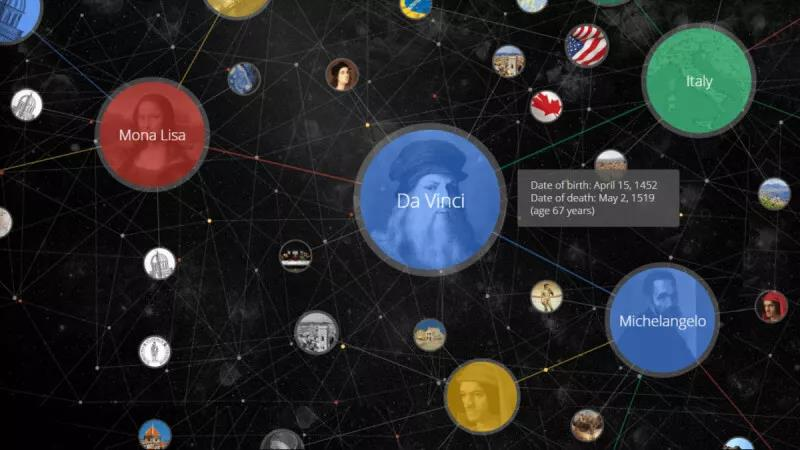
\includegraphics[width=0.56\textwidth]{KR20191218123426.jpg}
%    \label{KR20191218123426}
%\end{figure}
%%%%%%%%%%%%%%%%%%%%%%%%%%%%%%%%%%
%%%%%%%%%%%%%%%%%%%%%%%%%%%%%%%%%
\paragraph{知识表示的观点及方法}
%%%%%%%%%%%%%%%%%%%%%%%%%%%%%%%%%
\begin{itemize}
  \item 知识表示的观点
  \begin{itemize}
\item 陈述性观点: 知识的存储与知识的使用相分离.

           优点: 灵活、简洁, 演绎过程完整、确定, 知识维护方便.

           缺点: 推理效率低, 推理过程不透明.
\item 过程性观点: 知识寓于使用知识的过程中.

           优点: 推理效率高且推理过程清晰.

           缺点: 灵活性差且知识维护不便.
     \end{itemize}
\item 常用的知识表示方法
      \begin{itemize}
        \item \textbf{逻辑表示法}: 一阶谓词逻辑.
        \item \textbf{产生式表示法}: 产生式规则.
        \item \textbf{结构表示法}: 语义网络和框架.
        \item \textbf{过程表示法}: 将有关某一问题领域的知识, 连同如何使用这些知识的方法, 均隐式地表达为一个求解问题的过程.
      \end{itemize}
\end{itemize}
%%%%%%%%%%%%%%%%%%%%%%%%%%%%%%%%%
\section{一阶谓词逻辑表示法}
数理逻辑是一门研究推理的学科, 可分为:
%%%%%%%%%%%%%%%%%%%%%%%%%%%%%%%%%
\begin{itemize}
    \item \textbf{一阶经典逻辑}: 一阶经典命题逻辑, 一阶经典谓词逻辑. 命题逻辑和谓词逻辑是最先应用于人工智能的两种逻辑
    \item \textbf{非一阶经典逻辑}: 指除经典逻辑以外的那些逻辑, 例如: 二阶逻辑、多值逻辑和模糊逻辑等.
\end{itemize}

一阶谓词逻辑表示法是一种基于数理逻辑的表示方法.
\begin{itemize}
    \item 一阶谓词逻辑表示的逻辑学基础包括命题和真值; 论域和谓词;连词和量词; 项与合式公式; 自由变元与约束变元.
    \item 谓词逻辑表示方法: 是到目前为止能够表达人类思维活动规律的一种最精准形式语言. 它与人类的自然语言比较接近, 又可方便存储到计算机中去, 并被计算机进行精确处理.
    \item 谓词逻辑表示的应用和特性: 适于表示确定性的知识. 它具有自然性、精确性、严密性及易实现等特点.
\end{itemize}
%%%%%-------------------------------------%%%%%
\subsection{一阶谓词逻辑表示的逻辑学基础——命题与真值}
%%%%%%%%%%%%%%%%%%%%%%%%%%%%%%%%%
\begin{mydef}{断言}{1}
一个陈述句称为一个断言.
\end{mydef}
%%%%%%%%%%%%%%%%%%%%%%%%%%%%%%%%%
\begin{mydef}{命题}{1}
具有真假意义的断言称为命题.
\end{mydef}
%%%%%%%%%%%%%%%%%%%%%%%%%%%%%%%%%%%%
\begin{myprop}{命题真值}{1}
\begin{itemize}
    \item $T$: 表示命题的意义为真.
    \item $F$: 表示命题的意义为假.
        \begin{itemize}
            \item 一个命题不能同时既为真又为假.
            \item 一个命题可在一定条件下为真, 而在另一条件下为假.
        \end{itemize}
\end{itemize}
\end{myprop}

%%%%%-------------------------------------
\paragraph{论域和谓词}
\begin{itemize}
\item 论域: 由所讨论对象的全体构成的集合. 亦称为个体域.
\item 个体: 论域中的元素. 是命题的主语, 表示独立存在的事物或概念.
\item 谓词: 在谓词逻辑中, 命题是用形如$P(x_1,x_2,\cdots,x_n)$的谓词来表示的.
\item 谓词名: 是命题的谓语, 表示个体的性质、状态或个体之间的关系.
\end{itemize}

%%%%%-------------------------------------
\begin{mydef}{$n$元函数}{1}
     设$D$是个体域, $f: D^n\rightarrow D$是一个映射, 其中
\begin{align}
  D^{n}=\left\{\left(x_{1}, x_{2}, \cdots, x_{n}\right) | x_{1}, x_{2}, \cdots, x_{n} \in D\right\},
\end{align}
则称$f$是$D$上的一个$n$元函数, 记作$P(x_1,x_2,\cdots,x_n)$.
\end{mydef}

%%%%%-------------------------------------
\begin{mydef}{$n$元谓词}{1}
设$D$是个体域, $P: D^n\rightarrow \{T,F\}$是一个映射, 其中
\begin{align}
    D^{n}=\left\{\left(x_{1}, x_{2}, \cdots, x_{n}\right) | x_{1}, x_{2}, \cdots, x_{n} \in D\right\},
\end{align}
则称$P$是一个$n$元谓词, 记为$P(x_1,x_2,\cdots,x_n)$, 其中, $x_{1}, x_{2}, \cdots, x_{n}$为个体, 可以是个体常量、变元和函数.
\end{mydef}

%%%%%%%%%%%%%%%%%%%%%%%%%%%%%%%%%%
\begin{example}
GREATER($x,6$)表示$x$大于6.

\quad TEACHER(father(Wang Hong))表示王宏的父亲是一位教师.
\end{example}

谓词与函数的区别:
\begin{itemize}
\item 谓词是$D$到$\{T,F\}$的映射, 函数是$D$到$D$的映射.
\item 谓词的真值是$T$和$F$, 函数的值(无真值)是$D$中的元素.
\item 谓词可独立存在, 函数只能作为谓词的个体.
\end{itemize}
%%%%%----------------------------------------
\paragraph{连词}
\begin{itemize}
\item  $\neg$: “非”或者“否定”. 表示对其后面命题的否定.
\item  $\vee$: “析取”. 表示所连结的两个命题之间具有“或”的关系.
\item $\wedge$: “合取”.  表示所连结的两个命题之间具有“与”的关系.
\item $\rightarrow$: “条件”或“蕴含”. 表示“若…, 则…”的语义. 读作“如果$P$, 则$Q$”, 其中, $P$称为条件的前件, $Q$称为条件的后件.
\item $\leftrightarrow$: 称为“双条件”. 它表示“当且仅当”的语义. 即读作“$P$当且仅当$Q$”.
\end{itemize}
%%%%----------------------------------------------------
\begin{example}
对命题$P$和$Q$, $P \leftrightarrow Q$表示“$P$当且仅当$Q$”.
%%%%%--------------------------------------------------------------------------% tables and figures
\begin{table} [H]
\caption{真值表}
\vspace{-0.7cm}
\begin{center}
 \begin{tabular} {cccccccc}
  \hline
P	&Q&	$\neg$ P	&P$\vee$Q&	P$\wedge$Q	&P$\rightarrow$Q	&P$\leftrightarrow$Q\\
  \hline
T&  T&	F&	T&	T&	T&	T\\
T&	F&	F&	T&	F&	F&	F\\
F&	T&	T&	T&	F&	T&	F\\
F&	F&	T&	F&	F&	T&	T\\
\hline
\end{tabular}
\end{center}
\label{AI32_table1}
\end{table}
\end{example}
%%%%%%%%%%%%%%%%%%%%%%%%%%%%%%%
%%%%%----------------------------------------
\begin{mydef}{全称量词}{1}
全称量词, 意思是“所有的”、“任一个”.
\end{mydef}

\begin{itemize}
\item 命题($\forall x)P(x)$为真, 当且仅当对论域中的所有$x$, 都有$P(x)$为真.
\item 命题($\exists x)P(x)$为假, 当且仅当至少存在一个$x_i\in D$, 使得$P(x_i)$为假.

\quad $\bullet$ 存在量词, 意思是“至少有一个”或者“存在有”.
\item 命题($\exists  x)P(x)$为真, 当且仅当至少存在一个$x_i\in D$, 使得$P(x_i)$为真.
\item 命题($\forall x)P(x)$为假, 当且仅当对论域中的所有$x$, 都有$P(x)$为假.
\end{itemize}

%%%%%----------------------------------------
%%%%%%%%%%%%%%%%%%%%%%%%%%%%%%%%%%%%
\begin{myprop}{项满足的规则}{1}

    (1) 单独一个个体词是项;

    (2) 若$t_1,t_2,\cdots,t_n$是项, $f$是$n$元标量函数, 则$f(t_1,t_2,\cdots,t_n)$是项;

    (3) 由(1)和(2)生成的表达式是项.
\end{myprop}
%%%%%%%%%%%%%%%%%%%%%%%%%%%%%%%%%%%%
%%%%%%%%%%%%%%%%%%%%%%%%%%%%%%%%%%%%
\begin{myprop}{项}{1}
\textbf{项}是把个体常量、个体变量和函数统一起来的一个概念.
\end{myprop}
%%%%%%%%%%%%%%%%%%%%%%%%%%%%%%%%%%%%
\begin{mydef}{原子谓词公式}{1}
若$t_1,t_2,\cdots,t_n$是项, $P$是谓词, 则称$P(t_1,t_2,\cdots,t_n)$为\textbf{原子谓词公式}.
\end{mydef}
%%%%%%%%%%%%%%%%%%%%%%%%%%%%%%%%%%%%
%%%%%%%%%%%%%%%%%%%%%%%%%%%%%%%%%%%%
\begin{mydef}{合式公式}{1}
满足如下规则的谓词演算可得到合式公式:

    (1) 单个原子谓词公式是合式公式;

    (2) 若$A$是合式公式, 则$\neg A$也是合式公式;

    (3) 若$A,B$是合式公式, 则$A\vee B, A\wedge B, A\rightarrow B, A\leftrightarrow B$也都是合式公式;

    (4) 若$A$是合式公式, $x$是项, 则$(\forall x)A(x)$和$(\exists  x)A(x)$都是合式公式.
\end{mydef}
%%%%%%%%%%%%%%%%%%%%%%%%%%%%%%%%%%%%
\begin{example}
  $\neg P(x,y) \vee Q(y), (\forall x)(A(x)\rightarrow B(x))$, 都是合式公式.
\end{example}

连词的优先级(从高到低)
$$\neg,\wedge,\vee, \rightarrow,\leftrightarrow.$$

\begin{remark}
一般来说, 非”的优先级最高, 合取与析取以及其余几个的优先级用括号嵌套的表示方式区分.
\end{remark}

%%%%%----------------------------------------
\paragraph{自由变元与约束变元}
%%%%%%%%%%%%%%%%%%%%%%%%%%%%%%%%%%%%
\begin{itemize}
\item 辖域: 指位于量词后面的单个谓词或者用括弧括起来的合式公式.
\item 约束变元: 辖域内与量词中同名的变元称为约束变元.
\item 自由变元: 不受约束的变元称为自由变元.
\end{itemize}
%%%%%%%%%%%%%%%%%%%%%%%%%%%%%%%%例
\begin{example}
\begin{align}
  (\forall x)\textcolor[rgb]{0,0,1}{(}P(x,y)\rightarrow Q(x,y)\textcolor[rgb]{0,0,1}{)}\vee R(x, y),
\end{align}
其中, $P(x,y)\rightarrow Q(x,y)$是($\forall x$)的辖域.
\end{example}
%%%%%%%%%%%%%%%%%%%%%%%%%%%%%%%%
%%%%%%%%%%%%%%%%%%%%%%%%%%%%%%%%%%
\begin{myprop}{解释}{1}
辖域内的变元$x$是受($\forall$x)约束的变元, $R(x, y)$中的$x$和所有的$y$都是自由变元.
\end{myprop}

变元的换名: 谓词公式中的变元可以换名, 但需注意:
\begin{itemize}
\item 第一: 对约束变元, 必须把同名的约束变元都统一换成另外一个相同的名字, 且不能与辖域内的自由变元同名.
\item 第二: 对辖域内的自由变元, 不能改成与约束变元相同的名字.
\end{itemize}
%%%%%%%%%%%%%%%%%%%%%%%%%%%%%%%%例
\begin{example}
对($\forall x)P(x,y)$, 可把约束变元$x$换成$z$, 得到公式($\forall z)P(z, y)$.
\end{example}
%%%%%%%%%%%%%%%%%%%%%%%%%%%%%%%%例
\begin{example}
对($\forall x)P(x,y)$, 可把$y$换成$z$, 得到($\forall x)P(x,z)$ , 但不能换成$x$.
\end{example}
%%%%%%%%%%%%%%%%%%%%%%%%%%%%%%%%

表示步骤:

(1) 先根据要表示的知识定义谓词.

(2) 再用连词和量词把这些谓词连接起来.

%%%%%----------------------------------------
\paragraph{谓词逻辑表示方法}
%%%%%%%%%%%%%%%%%%%%%%%%%%%%%%%%例
\begin{example}
表示知识“所有教师都有自己的学生”.
\begin{itemize}
\item  定义谓词: $T(x)$: 表示$x$是教师.
               $S (y)$: 表示$y$是学生.
               $TS(x, y)$: 表示$x$是$y$的老师.
\item  表示知识($\forall x)(\exists y)(T (x)\rightarrow TS(x, y) \wedge S (y))$可读作: 对所有$x$, 如果$x$是一个教师, 那么一定存在一个个体$y$, $y$的老师是$x$, 且$y$是一个学生.
\end{itemize}
\end{example}
%%%%%%%%%%%%%%%%%%%%%%%%%%%%%%%%

%%%%%%%%%%%%%%%%%%%%%%%%%%%%%%%%例
\begin{example}
表示知识“所有的整数不是偶数就是奇数”.

定义谓词: $I(x)$: $x$是整数, $E(x)$: $x$是偶数,  $O(x)$: $x$是奇数.

表示知识: $(\forall x)(I(x) \rightarrow E(x)\vee O(x))$.
\end{example}
%%%%%%%%%%%%%%%%%%%%%%%%%%%%%%%%

%%%%%%%%%%%%%%%%%%%%%%%%%%%%%%%%例
\begin{example}
表示如下知识: 王宏是计算机系的一名学生. 王宏和李明是同班同学. 凡是计算机系的学生都喜欢编程序.
\begin{itemize}
\item 定义谓词:

COMPUTER$(x)$: 表示$x$是计算机系的学生.

CLASSMATE$(x,y)$: 表示$x$和$y$是同班同学.

LIKE$(x,y)$: 表示$x$喜欢$y$.

\item 表示知识:

COMPUTER(Wang Hong).

CLASSMATE(Wang Hong, Li Ming).

($\forall x$)(COMPUTER($x$)$\rightarrow$ LIKE($x$, programming)).
\end{itemize}

\end{example}
%%%%%%%%%%%%%%%%%%%%%%%%%%%%%%%%
%%%%%-----------------------------------------
\paragraph{谓词逻辑表示的应用}
%%%%%-----------------------------------------
\begin{example}(钱币翻转问)
设有三枚硬币,其初始状态为(反,正,反), 允许每次翻转一个硬币(只翻且必须翻一个硬币), 必须连翻三次. 问是否可以达到目标状态(正,正,正)或(反,反,反)?
\end{example}

\begin{answer}
用数组表示时, 显然每一硬币需占一维空间, 则用三维数组组成的状态向量表示这个知识: $Q=(q_1,q_2,q_3)$.
取$q=0$表示钱币的正面, $q=1$表示钱币的反面问题状态空间显然为$Q_0 =(0,0,0), Q_1=(0,0,1), Q_2=(0,1,0), Q_3=(0,1,1)$,
$Q_4=(1,0,0), Q_5=(1,0,1), Q_6=(1,1,0), Q_7=(1,1,1)$.

引入操作$a$: 把$q_1$翻一面. $b$: 把$q_2$翻一面. $c$: 把$q_3$翻一面. 显然$F=\{a,b,c\}$.
目标状态: $Q_g=(0,0,0)$或$Q_g=(1,1,1)$.
\end{answer}
%%%%%---------------------
\begin{figure}[!htp]
\centering
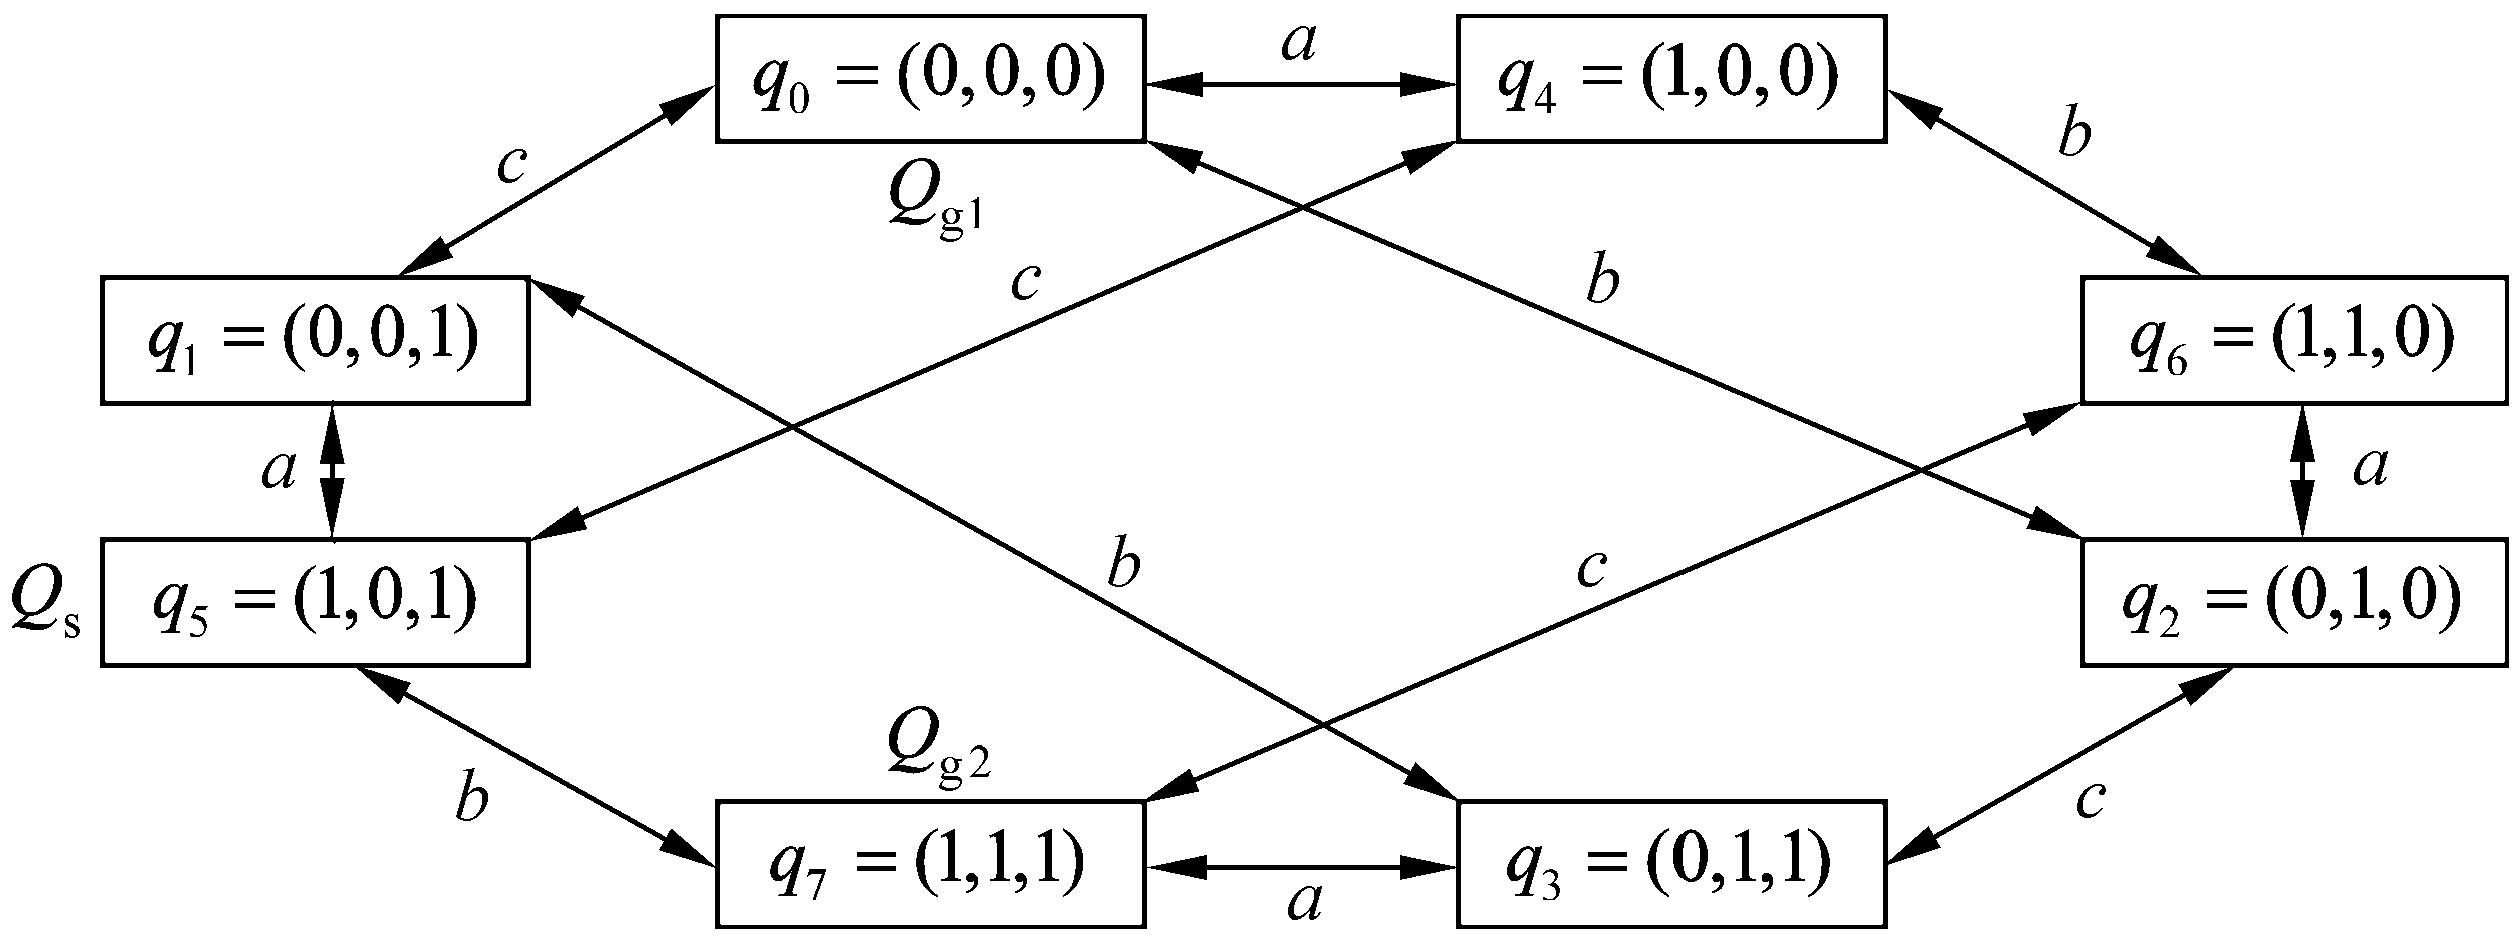
\includegraphics[width=0.6\textwidth]{MoneyStateSpace.jpg}
\caption{三枚钱币的状态空间图}
\label{MoneyStateSpacefig02}
\end{figure}

%%%%%-----------------------------------------
\begin{example}(机器人移盒子问题)
分别定义描述状态和动作的谓词.

1) 变元的个体域:
\begin{itemize}
\item 桌子$x$的个体域是$\{a, b\}$
\item 机器人$y$的个体域是$\{\textup{robot}\}$
\item 位置$z$的个体域是$\{a, b, c\}$
\item 盒子$w$的个体域是$\{\textup{box}\}$
\end{itemize}

2) 描述状态的谓词:
\begin{itemize}
\item TABLE($x$): $x$是桌子
\item EMPTY($y$): $y$手中是空的
\item AT($y, z$): $y$在$z$处
\item HOLDS($y, w$): $y$拿着$w$
\item ON($w, x$): $w$在$x$桌面上.
\end{itemize}

%%%%%-------------------------------------
\begin{minipage}{13.5cm}
{\quad 3) 问题的初始状态:}
\begin{minipage}{4.5cm}
\begin{itemize}
\item AT(robot, c)
\item EMPTY(robot)
\item ON(box, a)
\item TABLE(a)
\item TABLE(b)
\end{itemize}
\end{minipage}
%%%%%---------------------
\begin{minipage}{6cm}
\begin{figure}[H]
\centering
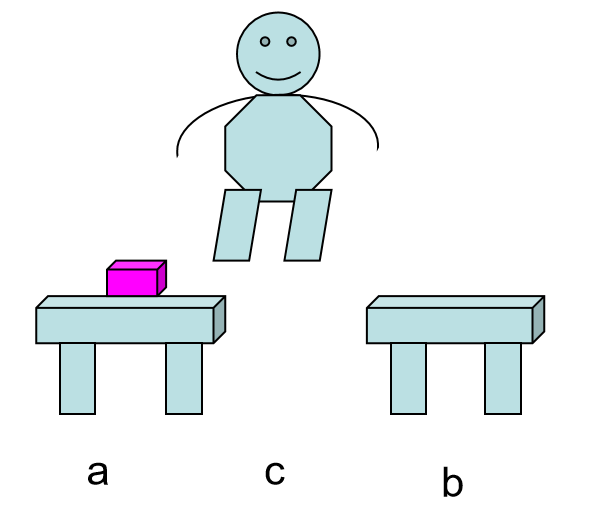
\includegraphics[width=0.65\textwidth]{RobotMoving2019112501.PNG}
\caption{机器人移盒子问题}
\label{AI32fig02}
\end{figure}
\end{minipage}
\end{minipage}
%%%%%-------------------------------------

\begin{minipage}{13.5cm}
{\quad 4) 问题的目标状态:}
\begin{minipage}{4.5cm}
\begin{itemize}
\item AT(robot, c)
\item EMPTY(robot)
\item ON(box, b)
\item TABLE(a)
\item TABLE(b)
\end{itemize}
\end{minipage}
\begin{minipage}{6cm}
\begin{figure}[H]
\centering
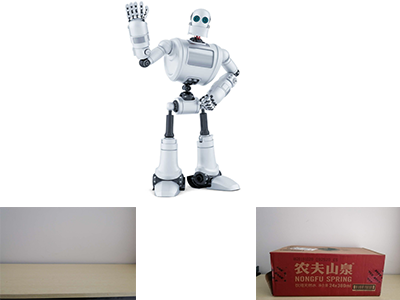
\includegraphics[width=0.65\textwidth]{RobotMoving2019112502.PNG}
\caption{机器人移盒子问题}
\label{AI32fig02}
\end{figure}
\end{minipage}
\end{minipage}
%\begin{figure}[htbp]
%\begin{center}
%\begin{tikzpicture}[font={\sf \small}]
%    \node (Gei) at (2,0) [draw, minimum height=0.25cm]{
\includegraphics[width=0.25\textwidth]{Desk01.jpg}};
%    \node (texta) [align=center,below=0.35cm of Gei]{$a$};
%    \node (ZCR1)[align=center,right=0.5cm of Gei,yshift=2cm] {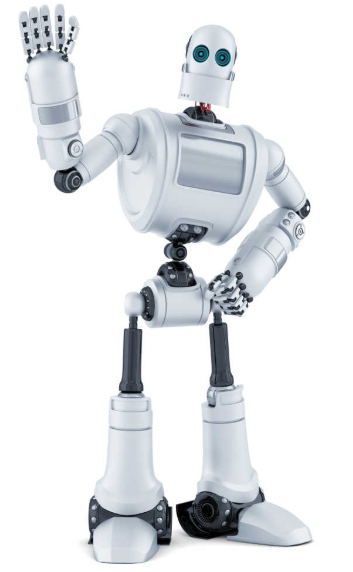
\includegraphics[width=0.2\textwidth]{Robot20202031901.PNG}};
%    \node (textb) [align=center,below=0.35cm of Gei,xshift=4cm]{$c$};
%    \node (TZCR1)[align=center,right=4.25cm of Gei,yshift=-1cm] {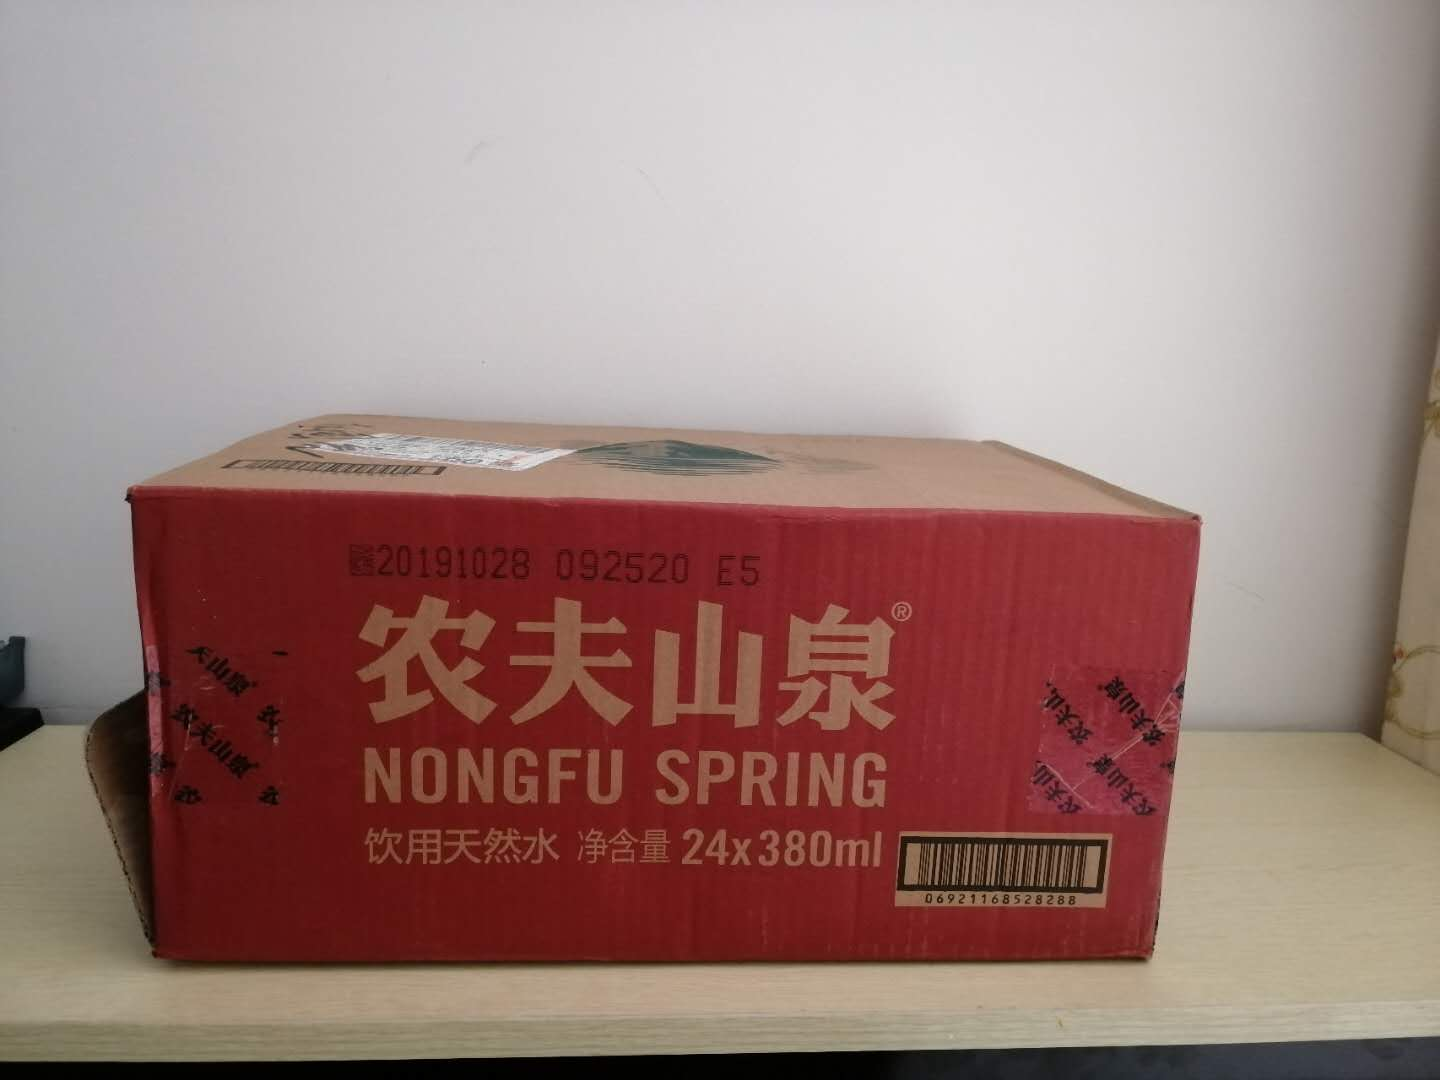
\includegraphics[width=0.20\textwidth]{Desk02.jpg}};
%    \node (textc) [align=center,below=0.35cm of Gei,xshift=8.25cm]{$b$};
%\end{tikzpicture}
%\end{center}
%\caption{机器人移盒子问题: }
%\label{AI32fig02}
%\end{figure}

机器人行动的目标把问题的初始状态转换为目标状态, 而要实现问题状态的转换需要完成一系列的中间操作.

5) 描述操作的谓词
\begin{itemize}
    \item 条件部分: 用来说明执行该操作必须具备的先决条件, 可用谓词公式来表示.
    \item 动作部分: 给出了该操作对问题状态的改变情况, 通过在执行该操作前的问题状态中删去和增加相应的谓词来实现.
\end{itemize}

6) 需要定义的操作:
\begin{itemize}
    \item Pickup($x$): 在$x$处拿起盒子.
    \item Goto($x, y$): 从$x$处走到$y$处.
    \item Setdown($x$): 在$x$处放下盒子.
\end{itemize}

7) 各操作的条件和动作:

\begin{itemize}
    \item Goto($x, y$)
    \begin{itemize}
        \item 条件: AT(robot, $x$).
        \item 动作: 删除表: AT(robot, $x$); 添加表: AT(robot, $y$).
    \end{itemize}
    \item Pickup(x).
    \begin{itemize}
        \item 条件: TABLE(x), ON(box, x), AT(robot, $x$), EMPTY(robot).
        \item 动作: 删除表: EMPTY(robot), ON(box, $x$); 添加表: HOLDS(robot, box).
    \end{itemize}
    \item Setdown($x$)
    \begin{itemize}
        \item 条件: AT(robot, $x$), TABLE($x$), HOLDS(robot, box).
        \item 动作: 删除表: HOLDS(robot, box; 添加表: EMPTY(robot), ON(box, $x$).
    \end{itemize}
\end{itemize}

    机器人每执行一操作前, 都要检查该操作的先决条件是否可以满足. 如果满足, 就执行相应的操作; 否则再检查下一个操作.
\end{example}
%%%%%-------------------------------------
\begin{answer}
机器人行动规划问题的求解过程:
\begin{itemize}
\item 状态1\,(初始状态)
          AT(robot, c), EMPTY(robot)$\xLongrightarrow{\quad \textup{开始} \quad}$ ON(box, a), TABLE(a), TABLE(b)
\item 状态2
          AT(robot, a), EMPTY(robot)$\xLongrightarrow{\textup{Goto(c, a)}}$ ON(box, a), TABLE(a), TABLE(b)
\item 状态3
        AT(robot, a), HOLDS(robot, box)$\xLongrightarrow{\textup{Pickup(a)}}$, TABLE(a), TABLE(b)
\item 状态4
       AT(robot, b), HOLDS(robot,box)$\xLongrightarrow{\textup{Goto(a, b)}}$, TABLE(a), TABLE(b)
\item 状态5
       AT(robot, b), EMPTY(robot)$\xLongrightarrow{\textup{Setdown(b)}}$, ON(box, b), TABLE(a), TABLE(b)
\item 状态6(目标状态)
         AT(robot, c), EMPTY(robot)$\xLongrightarrow{\textup{Goto(b, c)}}$, ON(box, b), TABLE(a), TABLE(b)
\end{itemize}
\end{answer}
%%%%%-----------------------------------------
\begin{figure}[htbp]
\vspace{-0.35cm}
\begin{center}
\begin{tikzpicture}[font={\sf\small},scale=0.8]
\def \smbwd{2cm}
\def \smbwe{4cm}
\node (Gei) at (2,0) [draw]{
\includegraphics[width=0.2\textwidth]{Monkeystempsnip.png}};
\node (texta) [align=center,below=0.35cm of Gei]{$a$};
\node (ZCR1)[align=center,right=0.5cm of Gei,yshift=2cm] {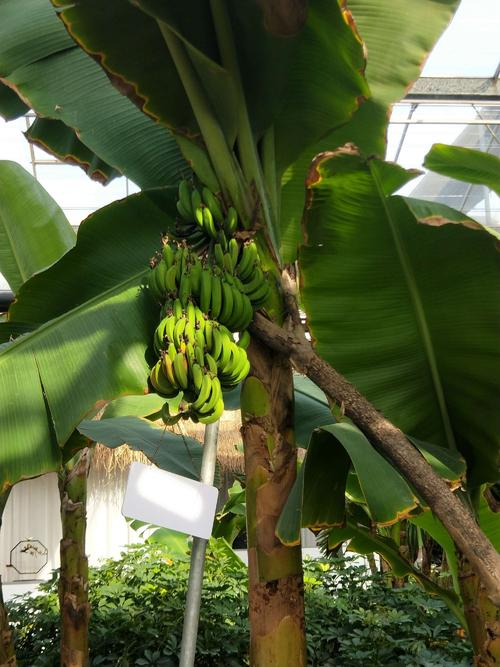
\includegraphics[width=0.15\textwidth]{BananaTree.jpg}};
\node (textb) [align=center,below=0.35cm of Gei,xshift=4cm]{$c$};
\node (TZCR1)[align=center,right=4.25cm of Gei,yshift=-0.6cm] {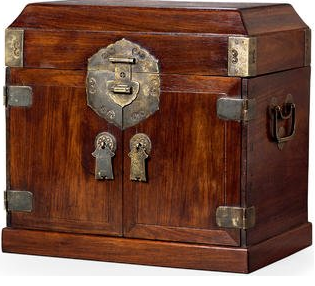
\includegraphics[width=0.20\textwidth]{Box0.png}};
\node (textc) [align=center,below=0.35cm of Gei,xshift=8.25cm]{$b$};
\end{tikzpicture}
\end{center}
\vspace{-0.75cm}
\caption{猴子摘香蕉问题}
\label{AI32fig03}
\end{figure}

\begin{example}(猴子摘香蕉问题, 图\ref{AI32fig03})
描述状态的谓词:
\begin{itemize}
\item AT($x, y$): $x$在$y$处.
\item ONBOX: 猴子在箱子上.
\item HB: 猴子得到香蕉.
\end{itemize}

\begin{itemize}
\item 个体域:

     $x$ : \{monkey, box, banana\}

     $Y: \{a, b, c\}$

\item 问题的初始状态

      AT(monkey, $a$)

      AT(box, $b$)

     $\neg$ ONBOX, $\neg$HB

\item 问题的目标状态

     AT(monkey, $c$), AT(box, $c$), ONBOX, HB
\end{itemize}
%%%%%-------------------------------------
描述操作的谓词
%%%%%-------------------------------------
\begin{itemize}
\item Goto($u, v$): 猴子从$u$处走到$v$处.
\item Pushbox($v, w$): 猴子推着箱子从$v$处移到$w$处.
\item Climbbox: 猴子爬上箱子.
\item Grasp: 猴子摘取香蕉.
\end{itemize}

各操作的条件和动作
\begin{itemize}
\item Goto($u, v$)

         条件: $\neg$ONBOX , AT(monkey, $u$),

         动作: 删除表: AT(monkey, $u$); 添加表: AT(monkey, $v$)
\item Pushbox($v, w$)

         条件:  $\neg$ ONBOX , AT(monkey, $v$), AT(box, $v$)

         动作: 删除表: AT(monkey, $v$), AT(box, $v$); 添加表: AT(monkey, $w$), AT(box,$w$)


\item Climbbox

          条件:  $\neg$ONBOX , AT(monkey, $w$), AT(box,$w$)

          动作: 删除表:  $\neg$ONBOX; 添加表: ONBOX
\item Grasp

         条件: ONBOX, AT(box, $c$)

         动作: 删除表:  $\neg$HB; 添加表: HB
\end{itemize}
\end{example}
%%%%%-------------------------------------
%\begin{figure}[H]
%\centering
%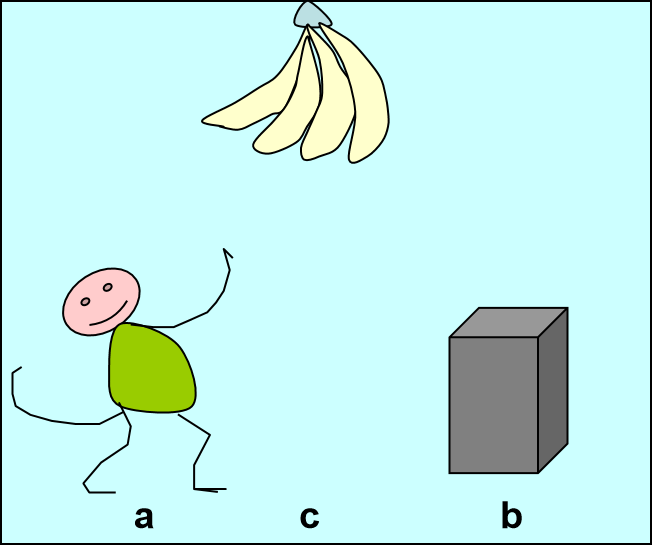
\includegraphics[width=0.46\textwidth]{Banana2019112502.PNG}
%\caption{猴子摘香蕉问题}
%\label{AI32fig03}
%\end{figure}


\begin{remark}
      一阶逻辑中,量词只能用于个体变元,取消这一限制条件,允许量词也可用于命题变元和谓词变元,由此构造起来的谓词逻辑就是高阶逻辑. 二阶逻辑是一阶逻辑的扩展, 一阶逻辑是命题逻辑的扩展. 公理化的高阶逻辑系统或高阶逻辑的自然推理系统又称为广义谓词演算或高阶谓词演算. 彭漪涟, 马钦荣, 《逻辑学大辞典》, 2010年上海辞书出版社.
\end{remark}

%%%%%-----------------------------------------
\subsection{谓词逻辑表示的特征}
%%%%%%%%%%%%%%%%%%%%%%%
\paragraph{谓词逻辑表示的主要优点}
\begin{itemize}
\item 自然: 一阶谓词逻辑是一种接近于自然语言的形式语言系统, 谓词逻辑表示法接近于人们对问题的直观理解.
\item 明确: 是一种标准的知识解释方法, 因此用这种方法表示的知识明确且易于理解.
\item 精确: 谓词逻辑的真值只有“真”与“假”, 其表示、推理都是精确的.
\item 灵活: 知识和处理知识的程序是分开的, 无须考虑处理知识的细节.
\item 模块化: 知识之间相对独立, 模块化的处理方式使得添加、删除和修改知识比较容易进行.
\end{itemize}
%%%%%%%%%%%%%%%%%%%%%%%%%%%%%%%%%%%%
\begin{myprop}{谓词逻辑的性质}{1}
\begin{itemize}
\item 自反性: $(\forall x)  R(x, x)$
\item 非自反性: $(\forall x)  \neg R(x, x)$
\item 传递性: $(\forall x) (\forall y) (\forall z)  [(R(x, y) \wedge R(y, z)) \rightarrow R(x, z)]$
\item  对称性: $(\forall x) (\forall y)  (R(x, y) \rightarrow R(y, x))$
\item 非对称性y: $(\forall x) (\forall y)  (R(x, y) \rightarrow \neg R(y, x))$
\item 反对称性: $(\forall x) (\forall y)  [(R(x, y) \wedge R(y, x)) \rightarrow x = y]$
\end{itemize}
\end{myprop}

%%%%%%%%%%%%%%%%%%%%%%%
\paragraph{主要缺点}
\begin{itemize}
\item 知识表示能力差: 只能表示确定性知识, 而\uwave{不能表示非确定性知识、过程性知识和启发式知识}.
\item 知识库管理困难: 缺乏知识的组织原则, 知识库管理比较困难.
\item 存在组合爆炸: 由于难以表示启发式知识, 因此只能盲目地使用推理规则, 这样当系统知识量较大时, 容易发生组合爆炸.
\item 系统效率低: 它把推理演算与知识含义截然分开, 抛弃了表达内容中所含有的语义信息, 往往使推理过程冗长, 降低了系统效率.
\end{itemize}

只考虑约束个体词的量词, 这种谓词逻辑就是一阶谓词逻辑. 带有两种量词的谓词逻辑,就是二阶逻辑.
自然语言的符号和自然语言之间的区别是语言学的研究对象, 不是逻辑学的研究对象.
在有些数学分支中比如拓扑学中, 需要二阶逻辑的能力来做完整的表达. 这方面的工作已经由 Stephen G. Simpson 在逆数学的名义下完成了.
已经证明了二阶逻辑不只对表达经典数学的某些重要部分是必须的, 而且它也可以用做模型论和数学基础的工具.

\begin{newexam}
\vspace{-0.2cm}
二阶句子
\begin{align}
    \forall S\forall x{\Big (}x\in S\vee x\notin S{\Big )},
\end{align}
对于所有个体的集合S和所有的个体x, 要么x在S中要么不在(这是二值原理)。最一般的二阶逻辑还包括量化在函数上的变量和解说变量.
\vspace{-0.2cm}
\end{newexam}

二阶逻辑比一阶逻辑更有表达力.
在二阶逻辑中, 有可能写出声称“论域是有限的”或“论域有可数势的”这样的形式句子. 要说论域是有限的, 可使用声称从论域到自身的所有单射函数都是满射的句子.
要声称论域有可数势, 可以使用声称在所有的论域的两个无限子集之间存在双射的句子.
从向上\href{https://zh.wikipedia.org/wiki/勒文海姆–斯科伦定理}{勒文海姆–斯科伦定理}得出在一阶逻辑内不可能特征化有限性或可数性.

\begin{newexam}
\vspace{-0.2cm}
在一阶逻辑中断言每个实数都有一个加法逆元:$\forall x \exists y(x + y = 0), x,y\in \mathbb R$, 需要二阶逻辑来断言实数的集合的上确界性质, 它声称实数的所有有界的、非空集合都有上确界. 如果论域是所有实数的集合, 表达了最小上界性质的二阶逻辑句子:
\begin{align}
  \forall A{\Big [}(\exists w(w\in A)&\land \exists z\,\forall w(w\in A\rightarrow w\leq z))\notag\\
                                     &\rightarrow \exists x\,\forall y([\forall w(w\in A\rightarrow w\leq y)]\leftrightarrow x\leq y){\Big ]}
\end{align}
\vspace{-0.2cm}
\end{newexam}

%%%%%-----------------------------------------
\subsection{知识表示——产生式表示法}
产生式(Production)是目前人工智能中使用最多的一种知识表示方法.

%    2.3.1 产生式表示的基本方法
%
%          事实的表示
%          规则的表示
%          产生式与蕴含式的区别
%          产生式与条件语句的区别
%
%    2.3.2 产生式系统的基本结构
%
%    2.3.3 产生式系统的基本过程
%
%    2.3.4 产生式系统的控制策略
%
%    2.3.5 产生式系统的类型
%
%    2.3.6 产生式系统的特性
%%%%%-----------------------------------------
\subsubsection{事实的表示}
%%%%%%%%%%%%%%%%%%%%%%%%%%%%%%%%%
\begin{mydef}{事实}{1}
    事实是断言一个语言变量或多个语言变量之间关系的陈述句.
\end{mydef}

\begin{remark}
    语言变量的值或语言变量之间的关系可以是数字和词等.
\end{remark}
%%%%%%%%%%%%%%%%%%%%%%%%%%%%%%%
\begin{example}
    “雪是白的”, 其中“雪”是语言变量, “白的”是语言变量的值.
    “王峰热爱祖国”, 其中, “王峰”和“祖国”是两个语言变量, “热爱”是语言变量之间的关系.
\end{example}
%%%%%-----------------------------------------
%%%%%%%%%%%%%%%%%%%%%%%%%%%%%%%
\begin{example}
    确定性知识, 事实可用如下三元组表示:
\begin{center}
    (对象, 属性, 值)或(关系, 对象1, 对象2)
\end{center}
其中,对象就是语言变量.

\begin{Verbatim}
    (snow, color, white) 或(雪, 颜色, 白)
    (love, Wang Feng, country) 或(热爱, 王峰, 祖国)
\end{Verbatim}

$\bullet$ 不确定性知识, 事实可用如下四元组表示:
\begin{center}
    (对象, 属性, 值, 可信度因子)
\end{center}
其中“可信度因子”是指该事实为真的相信程度. 可用$[0,1]$之间的一个实数来表示.
\end{example}
%%%%%-----------------------------------------
\subsection{规则的表示}
规则的作用是描述事物之间的因果关系.

%%%%------------------------------------
\begin{mydef}{产生式规则}{1}
    规则的产生式表示形式常称为产生式规则, 简称为产生式或规则.
\end{mydef}
%%%%%-----------------------------------------
\subparagraph{产生式的基本形式}
\begin{center}
  $P\rightarrow Q$  或者     IF  $P$  THEN $Q$,
\end{center}
其中, $P$是产生式的前提, 也称为前件, 它给出了该产生式可否使用的先决条件, 由事实的逻辑组合来构成;
$Q$是一组结论或操作, 也称为产生式的后件, 它指出当前题$P$满足时, 应该推出的结论或应该执行的动作.
%%%%%-----------------------------------------
\subparagraph{产生式的含义}
\begin{center}
    如果前提$P$满足, 则可推出结论$Q$或执行$Q$所规定的操作.
\end{center}
%%%%%-----------------------------------------
\subparagraph{产生式规则的例子}
\begin{center}
    $r_6$:  IF 动物有犬齿 AND 有爪 AND 眼盯前方   THEN 该动物是食肉动物,
\end{center}
其中, $r_6$是该产生式的编号; “动物有犬齿 AND 有爪 AND 眼盯前方”是产生式的前提$P$; “该动物是食肉动物”是产生式的结论$Q$.
%%%%%-----------------------------------------
\paragraph{产生式与蕴涵式、条件语句的区别}
\begin{itemize}
\item 与蕴涵式的主要区别:

     (1) 蕴涵式表示的知识只能是精确的, 产生式表示的知识可以是不确定的.

    \quad 原因是蕴涵式是一个逻辑表达式, 其逻辑值只有真和假.

     (2) 蕴含式的匹配一定要求是精确的, 而产生式的匹配可以是不确定的.

    \quad 原因是产生式的前提条件和结论都可以是不确定的, 因此其匹配也可以是不确定的.

\item 与条件语句的主要区别:

    (1) 前件结构不同

    \quad $\bullet$ 产生式的前件可以是一个复杂的结构.

    \quad $\bullet$ 传统程序设计语言中的左部仅仅是一个布尔表达式.

    (2) 控制流程不同

    \quad $\bullet$ 产生式系统中满足前提条件的规则被激活后, 不一定被立即执行, 规则能否执行将取决于冲突消解策略.
\end{itemize}
%%%%%-------------------------------------
\begin{remark}
    传统程序设计语言是严格地从一个条件语句向下一个条件语句传递.
\end{remark}
%%%%%-----------------------------------------
\subsection{产生式系统的基本结构——系统结构及说明}
%%%%%-----------------------------------------
\paragraph{综合数据库DB(Data Base)}
    存放求解问题的各种当前信息: \uwave{问题的初始状态、输入的事实、中间结论及最终结论等}.
    还能用于推理过程的规则匹配, 推理过程中, 当规则库中某条规则的前提可以和综合数据库的已知事实匹配时, 该规则被激活, 由它推出的结论将被作为新的事实放入综合数据库, 成为后面推理的已知事实.
%%%%%-----------------------------------------
\begin{mydef}{规则库RB(Rule Base)}{1}
    也称知识库KB(Knowledge Base), 用于存放与求解问题有关的所有规则的全体.
\end{mydef}
\begin{itemize}
    \item 作用: 是产生式系统问题求解的基础.
    \item 要求: 知识的完整性、一致性、准确性、灵活性和知识组织的合理性.
\end{itemize}
%%%%%-------------------------------------
%\begin{figure}[H]
%\centering
%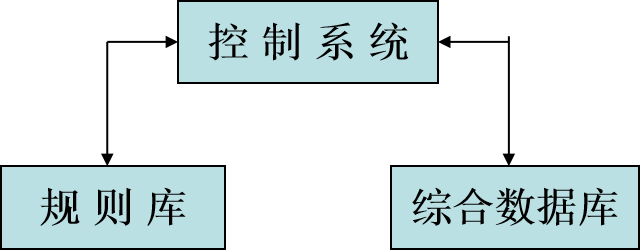
\includegraphics[width=0.5\textwidth]{tuiliguize2019112505.PNG}
%\caption{产生式系统的基本结构}
%\label{AI32fig05}
%\end{figure}
%%%%%%%%%%%%%%%%%%%%%%%%%%%%%%%
\begin{figure}[H]
\begin{center}
\begin{tikzpicture}[font={\sf \small}]
\def \smbwd{2cm}
\def \smbwe{4cm}
\thispagestyle{empty}
%定义流程图的具体形状
\node (qLPV) at (0,0) [draw, process,minimum width=\smbwd, minimum height=0.5cm] {控制系统};       % 控制系统
\node (RB0)[draw, process,align=center,below=2cm of qLPV,xshift=-3cm] {规则库};             % 规则库
\node (SDB0)[draw, process,align=center,below=2cm of qLPV,xshift=3cm] {综合数据库};         % 综合数据库
\draw[thick, <->] (qLPV.west)-|(RB0)node[left,yshift=0.25cm,xshift=-1cm] {};
\draw[thick,<->] (qLPV.east)-|(SDB0)node[left,yshift=0.25cm,xshift=-1cm] {};
\end{tikzpicture}
\caption{产生式系统的基本结构}
\label{AI32fig05}
\end{center}
\end{figure}
%%%%%-------------------------------------
%%%%%-----------------------------------------
\paragraph{控制系统(Control system)}
%%%%%-----------------------------------------
\subparagraph{控制系统}
    亦称推理机, 主要作用是控制整个产生式系统的运行, 决定问题求解过程的推理线路.
%%%%%-----------------------------------------
\subparagraph{控制系统的主要任务}
\begin{itemize}
\item \textbf{选择匹配}: 按一定策略从规则库中选择规则与综合数据库中的已知事实进行匹配. 匹配是指把所选规则的前提与综合数据库中的已知事实进行比较, 若事实库中存的事实与所选规则前提一致, 则称\textbf{匹配成功}, 该规则可用;否则, 称匹配失败, 该规则不可用.
\item \textbf{冲突消解}: 对匹配成功的规则, 按照某种策略从中选出一条规则执行.
\item \textbf{执行操作}: 对所执行的规则, 若其后件为一个或多个结论, 则把这些结论加入综合数据库;若其后件为一个或多个操作时, 执行这些操作.
\item \textbf{终止推理}: 检查综合数据库中是否包含有目标, 若有, 则停止推理.
\item \textbf{路径解释}: 在问题求解过程中, 记住应用过的规则序列, 以便最终能够给出问题的解路径.
\end{itemize}

%%%%%%%%%%%%%%%%%%%%%%%%%%%%%%%%产生式系统的例子
\begin{example}
    \textbf{动物识别系统}: 该系统可以识别老虎、金钱豹、斑马、长颈鹿、企鹅和信天翁这6种动物. 其规则库包含如下15条规则:
\begin{itemize}
\item $r_{1}$   IF   该动物有毛发   THEN   该动物是哺乳动物
\item $r_{2}$   IF   该动物有奶    THEN   该动物是哺乳动物
\item $r_{3}$   IF   该动物有羽毛  THEN   该动物是鸟
\item $r_{4}$   IF   该动物会飞  AND  会下蛋  THEN  该动物是鸟
\item $r_{5}$   IF   该动物吃肉   THEN   该动物是食肉动物
\item $r_{6}$   IF   该动物有犬齿  AND  有爪   AND   眼盯前方
                          THEN   该动物是食肉动物
\item $r_{7}$   IF  该动物是哺乳动物  AND  有蹄  THEN  该动物是有蹄类动物
\item $r_{8}$   IF 该动物是哺乳动物 AND 是嚼反刍动物 THEN 该动物是有蹄类动物
\item $r_{9}$   IF 该动物是哺乳动物  AND  是食肉动物 AND  是黄褐色
          AND  身上有暗斑点  THEN   该动物是金钱豹

\item $r_{10}$  IF  该动物是哺乳动物   AND  是食肉动物   AND  是黄褐色
          AND  身上有黑色条纹  THEN   该动物是虎
\item $r_{11}$  IF   该动物是有蹄类动物   AND  有长脖子  AND  有长腿
          AND  身上有暗斑点  THEN   该动物是长颈鹿
\item $r_{12}$  IF  动物是有蹄类动物 AND 身上有黑色条纹 THEN 该动物是斑马
\item $r_{13}$  IF   该动物是鸟  AND  有长脖子  AND  有长腿  AND  不会飞
          AND  有黑白二色    THEN   该动物是鸵鸟
\item $r_{14}$  IF   该动物是鸟  AND  会游泳  AND  不会飞   AND  有黑白二色
                              THEN   该动物是企鹅
\item $r_{15}$  IF   该动物是鸟   AND   善飞   THEN   该动物是信天翁,

其中, $r_i(i=1,2,\cdots,15)$是规则的编号.

\textbf{初始综合数据库包含的事实有:动物有暗斑点, 有长脖子, 有长腿, 有奶, 有蹄.}
\end{itemize}
\end{example}

系统的推理过程

(1) 先从规则库中取出第一条规则$r_1$, 检查其前提是否可与综合数据库中的已知事实相匹配. $r_1$的前提是“有毛发”, 但事实库中无此事实, 故匹配失败. 然后取$r_2$, 该前提可与已知事实“有奶”相匹配, $r_2$被执行,
并将其结论“该动物是哺乳动物”作为新的事实加入到综合数据库中. 此时, 综合数据库的内容变为:
\begin{center}
    动物有暗斑, 有长脖子, 有长腿, 有奶, 有蹄, \textcolor[rgb]{0,0,1}{是哺乳动物}.
\end{center}

(2) 再从规则库中取$r_3,r_4,r_5,r_6$进行匹配, 均失败. 接着取$r_7$, 该前提与已知事实“是哺乳动物”相匹配, $r_7$被执行, 并将其结论“该动物是有蹄类动物” 作为新的事实加入到综合数据库中. 此时, 综合数据库的内容变为:
\begin{center}
    动物有暗斑, 有长脖子, 有长腿, 有奶, 有蹄, 是哺乳动物, \textcolor[rgb]{0,0,1}{是有蹄类动物}.
\end{center}

(3) 此后, $r_8,r_9,r_{10}$均匹配失败. 接着取$r_{11}$, 该前提 “该动物是有蹄类动物  AND  有长脖子  AND  有长腿  AND  身上有暗斑” 与已知事实相匹配, $r_{11}$被执行, 并推出“\textcolor[rgb]{1,0,0}{该动物是长颈鹿}”. 由于“长颈鹿”已是目标集合中的一个结论, 即已推出最终结果, 故问题求解过程结束.

该例子的部分推理网络如图\ref{AI32fig06}, 图\ref{AI32fig06}中最上层的结点称为“假设”或“结论”.中间节点称为“中间假设”; 终结点称为“证据”或“事实”; 每个“结论”都是本问题的一个目标, 所有“假设”构成了本问题的目标集合.
%%%%%-------------------------------------
\begin{figure}[H]
    \centering
    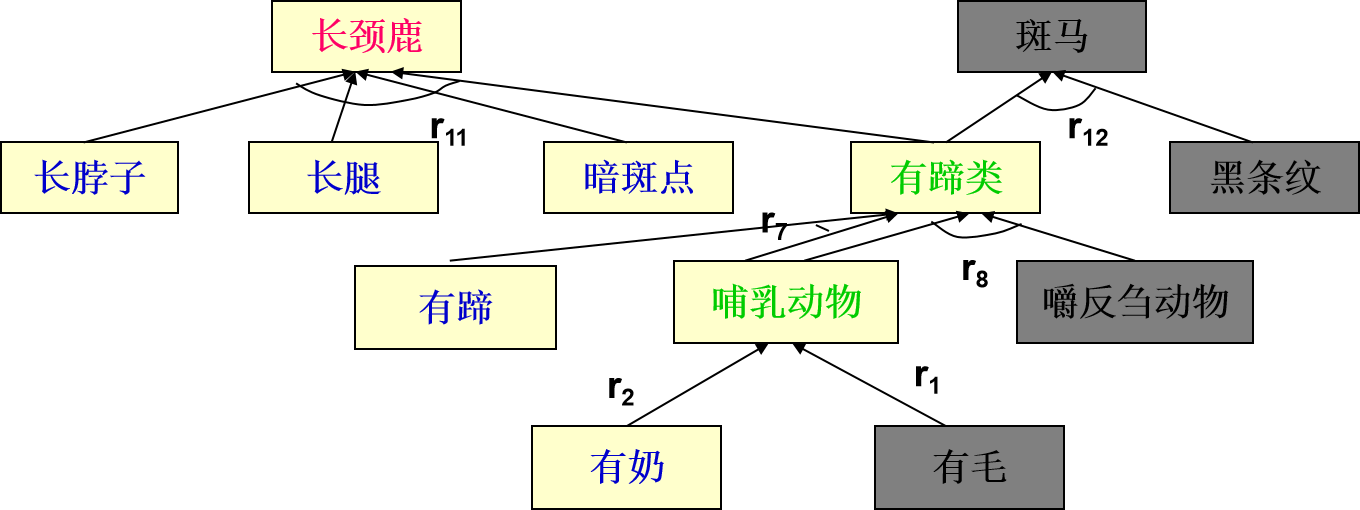
\includegraphics[width=0.6\textwidth]{Chanshengshi2019112506.PNG}
    \caption{产生式系统的推理结果}
    \label{AI32fig06}
\end{figure}
%%%%%-------------------------------------
\begin{remark}
    上述规则仅是一种直接表示方式, 用三元组表示$r_{15}$如下:
\begin{center}
  $r_{15}$: \,\,\textup{IF}\,\,(动物, 类别, 鸟)AND(动物, 本领, 善飞)\,\,\textup{THEN}\,\,(动物, 名称, 信天翁).
\end{center}
\end{remark}
%%%%%-----------------------------------------
\subsection{产生式系统的过程——基本过程}

(1) 初始化综合数据库, 把待解决问题的已知事实整理并送入综合数据库中;

(2) 检查规则库中是否有未使用过的规则, 若无, 转 (7);

(3) 检查规则库中未使用规则是否有其前提可与综合数据库中已知事实相匹配的规则, 若有, 形成当前可用规则集;否则, 转(6);

(4) 按照冲突消解策略, 从当前可用规则集中选择一个规则执行, 并对该规则作上标记. 把执行该规则后所得到的结论作为新的事实放入综合数据库;如果该规则的结论是一些操作, 则执行这些操作;

(5) 检查综合数据库中是否包含了该问题的解, 若已包含, 说明解已求出, 问题求解过程结束; 否则, 转(2);

(6) 当规则库中还有未使用规则, 但均不能与综合数据库中的已有事实相匹配时, 要求用户进一步提供关于该问题的已知事实, 若能提供, 则转(2); 否则, 执行下一步;

(7) 若知识库中不再有未使用规则, 也说明该问题无解, 终止问题求解过程.
%%%%%-------------------------------------
\begin{remark}
  从第(3)步到第(5)步的循环过程实际上就是一个\textbf{搜索过程}.
\end{remark}

%%%%------------------------------------%
总体上可分为以下两种方式

1) 不可撤回方式

\begin{itemize}
    \item 是一种“一直往前走”不回头的方式, 类似于中国象棋中过河的卒子.
    它即根据当前已知的局部知识选取一条规则作用于当前综合数据库, 接着再根据新状态继续选取规则, 如此进行下去, 不考虑撤回用过的规则.不理想规则的应用会降低效率, 但不影响可解性.
\end{itemize}

\textbf{优点}是控制过程简单, 缺点是当问题有多个解时不一定能找到最优解.

2) 试探性方式, 可分为以两种下方式:
\begin{itemize}
    \item 回溯方式是一种碰壁回头的方式. 即在问题求解过程中, 允许先试一试某条规则, 如果以后发现这条规则不合适, 则允许退回去, 再另选一条规则来试.

          需要解决的主要问题: 一是如何确定回溯条件, 二是如何减少回溯次数. 是一种完备而有效的策略, 它容易实现且占内存容量较小.

    \item 图搜索方式

         图搜索方式是一种用图或树把全部求解过程记录下来的方式. 由于它记录了已试过的所有路径, 因此便于从中选取最优路径.
\end{itemize}
%%%%------------------------------------%
\begin{remark}
\textbf{主要区别}: 回溯方式抹去了所有引起失败的试探路径, 而图搜索方式则记住了已试过的所有路径.
\end{remark}
%%%%%-----------------------------------------
\paragraph{按推理方向}
\begin{itemize}
\item \textbf{正向推理产生式系统}, 也称数据驱动方式, 它是从初始状态出发, 朝着目标状态前进, 正向使用规则的一种推理方法.
%%%%%-------------------------------------
\begin{remark}
所谓正向使用规则, 是指以问题的初始状态作为初始综合数据库, 仅当综合数据库中的事实满足某条规则的前提时, 该规则才被使用.
\end{remark}

$\bullet$ \textbf{优点}: 简单明了, 且能求出所有解.

$\bullet$ \textbf{缺点}: 执行效率较低, 原因是使用规则具有一定的盲目性.

\item \textbf{逆向推理产生式系统}, 也称目标驱动方式, 它是从目标(作为假设)状态出发, 朝着初始状态前进, 逆向使用规则的一种推理方法.
%%%%%-------------------------------------
\begin{remark}
    所谓逆向使用规则, 是指以问题的目标状态作为初始综合数据库, 仅当综合数据库中的事实满足某条规则的后件时, 该规则才被使用 .
\end{remark}

$\bullet$ \textbf{优点}: 不使用与问题无关的规则. 因此, 对那些目标明确的问题, 使用逆向推理方式是一种最佳选择.

\item \textbf{双向推理产生式系统}, \textbf{双向推理}是把正向推理和反向推理结合起来使用的一种推理方式. 它需要把问题的初始状态和目标状态合并到一起构成综合数据库.
\end{itemize}
%%%%%-----------------------------------------
\paragraph{按规则库的性质及结构}
%%%%%-----------------------------------------
\begin{itemize}
\item \textbf{可交换的产生式系统}是一种对规则的使用次序无关的产生式系统, 即任意交换规则的使用次序都不会影响对问题的求解.

\quad 假设$DB$是综合数据库, $RB$是规则库, $DB_i (i=1,2,\cdots)$是第$i$次使用规则后得到的新的综合数据库, $RS$是一个可作用于$DB_i$的规则集合. 若一个产生式系统可交换, 则其$RB$和每一个$DB_i$都应具有如下性质:

    \quad\ding{172} 对任一规则$r_j=RS (j=1,2,\cdots)$, 它作用于$DB_i$得到新的综合数据库$DB_{i+1}$, RS仍然是$DB_{i+1}$的可用规则集.

    \quad\ding{173}  如果$DB_i$满足目标条件, 则用RS中的任一规则$r_j$作用于$DB_i$, 得到的$DB_{i+1}$仍然满足目标条件.

    \quad\ding{174}  若对$DB_i$使用某一规则序列$r_1,r_2,\cdots,r_k$得到一个新的综合数据库$DB_k$, 则当改变这些规则的使用次序后, 仍然可得到$DB_k$.

\quad 可见, 综合数据库是递增的, 即对任何序列$r_1,r_2,\cdots,r_g$, 其作用于DB 后所得到的$DB_1,DB_2,\cdots,DB_g$之间存在如下关系:
\begin{center}
  $DB_1\subset  DB_2\subset  \cdots\subset DB_g$.
\end{center}
%%%%%-------------------------------------
\begin{remark}
  这说明在可交换产生式系统中, 其规则的结论部分总是包含着新的内容, 一旦执行该规则就会把这些新的内容添加到综合数据库中.
\end{remark}

%%%%%---------------------------------------------
\begin{example}
  设给定一个整数集合$\{a,b,c\}$, 可通过把集合中任意一对元素的乘积作为新元素添加到集合中的办法来扩大该整数集, 要求通过若干次操作后能生成所需的整数集合.
\end{example}
综合数据库$DB$可用集合来表示

\item 初始状态为$\{a,b,c\}$;
\item 目标状态为${a, b, c, a\times b, b\times c, a\times c}$;
\item 规则库RB中包含的规则有:

    \quad$r_1$:\,\,   IF\,\,      $\{a,b,c\}$\,\,      THEN \,\,      $\{a, b, c, a\times b \}$

    \quad$r_2$:\,\,      IF \,\,     $\{a,b,c\}$\,\,      THEN\,\,       $\{a, b, c, b\times c\}$

     \quad$r_3$:\,\,      IF\,\,     $\{a,b,c\}$\,\,     THEN\,\,       $\{a, b, c, a\times c\}$

      显然, 无论先使用哪一条规则都可由初始状态达到目标状态. 因此, 上述由DB和RB所构造的产生式系统是一个可交换的产生式系统, 并具有可交换产生式系统三个性质.

\quad 可交换产生式系统的可交换性, 使得其求解过程只需要搜索其中的任意一条路经, 就能达到目标, 而不必进行回溯.
      这种系统的求解过程可采用不可撤回的控制方式.

\item \textbf{可分解的产生式系统}

     把一个整体问题分解成若干个子问题, 然后再通过对这些子问题的求解来得到整个问题解的一种产生式系统.
\end{itemize}
%%%%------------------------------------%%
\begin{example}
设综合数据库的初始状态为$\{C, B, Z\}$, 目标状态为$\{M, M,\cdots, M\}$, 规则库中有如下重写规则:
\begin{itemize}
\item $r_1$: C$\rightarrow$\{D, L\}.
\item $r_2$: C$\rightarrow$\{B, M\}.
\item $r_3$: B$\rightarrow$\{M, M\}.
\item $r_4$: Z$\rightarrow$\{B, B, M\}.
\end{itemize}
\end{example}
解决该问题时, 可先把初始综合数据库分为三个子库, 然后对这三个子库分别应用规则库中的相应规则进行求解. 其求解过程如图\ref{AI32fig07}所示.
%%%%%-----------------------------------------
\subparagraph{可恢复的产生式系统}
%%%%%-------------------------------------
\begin{figure}[H]
\vspace{-0.5cm}
\centering
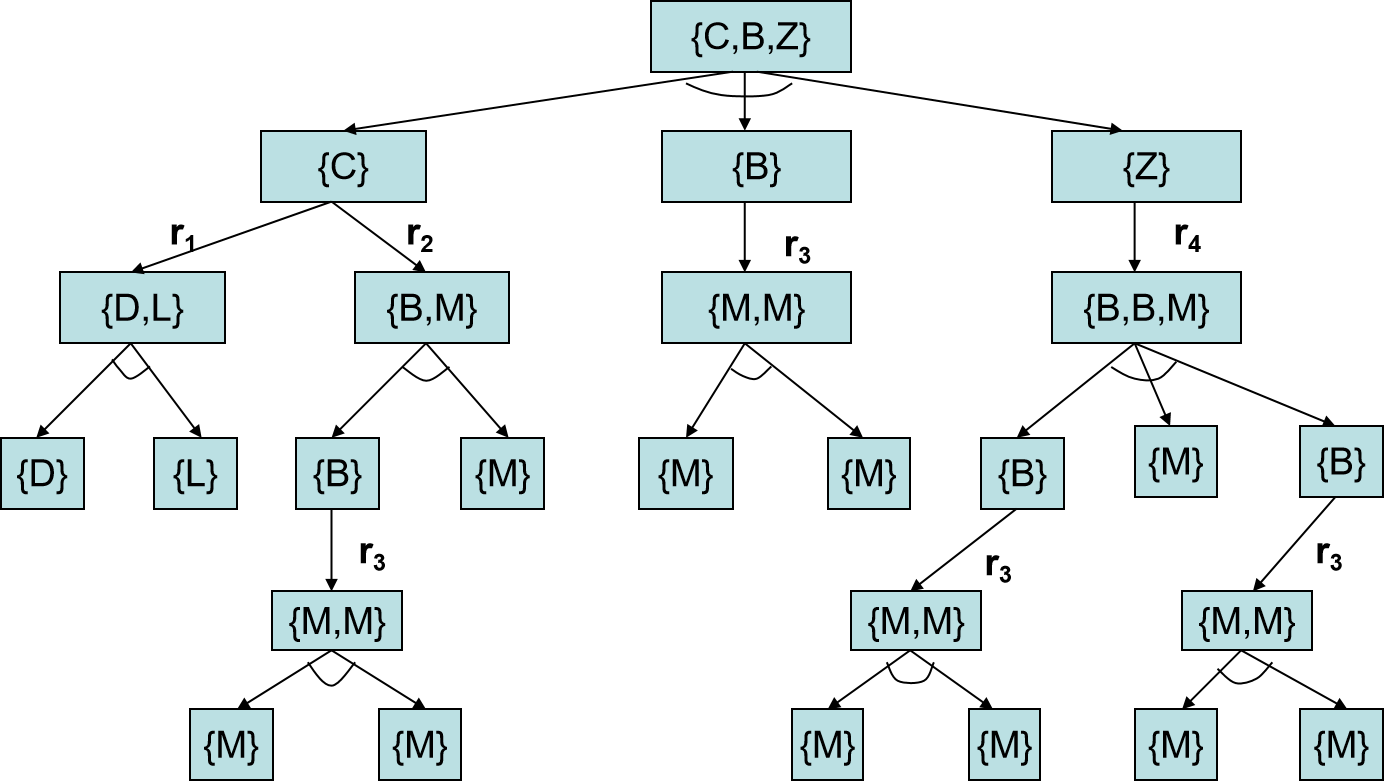
\includegraphics[width=0.6\textwidth]{Chanshengshiiegou2019112506.PNG}
\caption{按规则库的性质及结构}
\label{AI32fig07}
\end{figure}
%%%%%-------------------------------------
\begin{itemize}
\item 是指那种采用回溯控制方式的产生式系统.
\item 其求解问题的方法是: 当执行某条规则后, 如果发现所得到的新的综合数据库不可能求出问题的解, 就立即撤消由该规则所产生的结果, 使综合数据库恢复到先前的状态, 然后再另选别的规则继续求解.
\item 它既可以向综合数据库中添加新的内容, 又可以从综合数据库中删除或修改老的内容. 这种求解问题的方法, 更符合人们的一般习惯.
\item 对可恢复的产生式系统, 也将在第\ref{AIchap4}章详细讨论.
\end{itemize}
%%%%%-----------------------------------------
\subsection{产生式系统的特点}
%%%%%-----------------------------------------
\paragraph{主要优点}
\begin{itemize}
\item 自然性: 采用“如果$\cdots\cdots$, 则$\cdots\cdots$”的形式, 人类的判断性知识基本一致.
\item 模块性: 规则是规则库中最基本的知识单元, 各规则之间只能通过综合数据库发生联系, 而不能相互调用, 从而增加了规则的模块化程度.
\item 有效性: 产生式知识表示法既可以表示确定性知识, 又可以表示不确定性知识, 既有利于表示启发性知识, 又有利于表示过程性知识.
\item 一致性: 规则库中的所有规则都具有相同的格式, 并且综合数据库可被所有规则访问, 因此规则库中的规则可以统一处理.
\end{itemize}
%%%%%-----------------------------------------
\paragraph{主要缺点}
\begin{itemize}
\item 效率较低: 各规则之间的联系必须以综合数据库为媒介. 求解过程是一种反复进行的“\uwave{匹配—冲突消解—执行}”过程. 这样的执行方式将导致执行的效率低.
\item 不便于表示结构性知识: 由于产生式表示中的知识具有一致格式, 且规则之间不能相互调用, 因此那种具有结构关系或层次关系的知识则很难以自然的方式来表示.
\end{itemize}
%%%%%-----------------------------------------
\section{语义网络表示法}
语义网络是奎廉(J. R. Quillian) 1968年在研究人类联想记忆时提出的一种心理学模型, 认为记忆是由概念间的联系实现的.
随后, 奎廉又把它用作知识表示.
1972年, 西蒙在他的自然语言理解系统中也采用了语义网络表示法.
1975年, 亨德里克(G. G. Hendrix)又对全称量词的表示提出了语义网络分区技术.
%%%%%-----------------------------------------
\subsection{语义网络}
\subsubsection{语义网络}
\begin{mydef}{语义网络}{1}
语义网络是一种用实体及其语义关系来表达知识的有向图.
结点代表实体, 表示各种事物、概念、情况、属性、状态、事件和动作等;
弧代表语义关系, 表示它所连结的两个实体之间的语义联系, 它必须带有标识.
\end{mydef}
%%%%%-----------------------------------------
\begin{mydef}{语义基元}{1}
    语义网络中最基本的语义单元称为语义基元, 可用三元组表示为:
\begin{center}
    (结点1, 弧, 结点2)
\end{center}
\end{mydef}
%%%%%-----------------------------------------
\paragraph{基本网元}
    指一个语义基元对应的有向图.
%%%%------------------------------------%%
\begin{example}
    若有语义基元$(A, R, B)$, 其中, $A,B$分别表示两个结点, $R$表示$A$与$B$之间的某种语义联系, 对应的基本网元如图\ref{AI32fig000021}所示:
%%%%%%%%%%%%%%%%%%%%%%%%%%%%%%
\begin{figure}[H]
\begin{center}
\begin{tikzpicture}[font={\sf \small}]
\def \smbwd{2cm}
\def \smbwe{4cm}
\thispagestyle{empty}
%定义流程图的具体形状
\node (qLPV) at (0,0) [draw, process,minimum width=\smbwd, minimum height=0.5cm] {A};      % 李刚
\node (UniSampling)[draw, process,align=center,right=2cm of qLPV,yshift=0cm] {B};           %人
\draw[->] (qLPV.east)->(UniSampling)node[left,yshift=0.25cm,xshift=-1cm] {R};
\end{tikzpicture}
\caption{语义联系的基本网元}
\label{AI32fig000021}
\end{center}
\end{figure}
%%%%%%%%%%%%%%%%%%%%%%%%%%%%%%
\end{example}
%%%%%-------------------------------------
%%%%%-----------------------------------------
\subparagraph{语义网络的简单例子}
%%%%------------------------------------%%
\begin{example}
    用一网络表示“鸵鸟是一种鸟”.
\end{example}
%%%%%%%%%%%%%%%%%%%%%%%%%%%%%%
\begin{figure}[H]
\begin{center}
\begin{tikzpicture}[font={\sf \small}]
\def \smbwd{2cm}
\def \smbwe{4cm}
\thispagestyle{empty}
%定义流程图的具体形状
\node (qLPV) at (0,0) [draw, process,minimum width=\smbwd, minimum height=0.5cm] {鸵鸟};      % 鸵鸟
\node (UniSampling)[draw, process,align=center,right=2cm of qLPV,yshift=0cm] {鸟};            % 鸟
\draw[->] (qLPV.east)->(UniSampling)node[left,yshift=0.25cm,xshift=-0.6cm] {是一种};
\end{tikzpicture}
\caption{语义联系的基本网元}
\label{AI32fig000022}
\end{center}
\end{figure}
%%%%%%%%%%%%%%%%%%%%%%%%%%%%%%
语义网络与产生式对应的表示能力.
%%%%%-----------------------------------------
\paragraph{事实的表示}
%%%%------------------------------------%%
\begin{example}
    “雪的颜色是白的”.
\end{example}
%%%%%%%%%%%%%%%%%%%%%%%%%%%%%%
\begin{figure}[H]
\begin{center}
\begin{tikzpicture}[font={\sf \small}]
\def \smbwd{2cm}
\def \smbwe{4cm}
\thispagestyle{empty}
%定义流程图的具体形状
\node (qLPV) at (0,0) [draw, process,minimum width=\smbwd, minimum height=0.5cm] {雪};      % 雪
\node (UniSampling)[draw, process,align=center,right=2cm of qLPV,yshift=0cm] {白};           %白
\draw[->] (qLPV.east)->(UniSampling)node[left,yshift=0.25cm,xshift=-0.9cm] {颜色};
\end{tikzpicture}
\caption{语义联系的基本网元}
\label{AI32fig000022}
\end{center}
\end{figure}
%%%%%%%%%%%%%%%%%%%%%%%%%%%%%%
%%%%%-----------------------------------------
\paragraph{规则的表示}
%%%%------------------------------------%%
\begin{example}
  规则R的含义是“如果   A\, 则    B ”.
\end{example}
%%%%%-----------------------------------------
\paragraph{基本的语义关系}
主要分8种关系, 包括\uwave{实例关系、分类关系、成员关系、属性关系、聚类关系、时间关系、位置关系和相近关系}.
%%%%%-----------------------------------------
\subparagraph{1) 实例关系: ISA}
体现的是“具体与抽象”的概念, 含义为“是一个”, 表示一个事物是另一个事物的一个实例.
%%%%%-------------------------------------
\begin{example}ISA例子
\begin{figure}[H]
\begin{center}
\begin{tikzpicture}[font={\sf \small}]
\def \smbwd{2cm}
\def \smbwe{4cm}
\thispagestyle{empty}
%定义流程图的具体形状
\node (qLPV) at (0,0) [draw, process,minimum width=\smbwd, minimum height=0.5cm] {李刚};      % 李刚
\node (UniSampling)[draw, process,align=center,right=2cm of qLPV,yshift=0cm] {人};            %人
\draw[->] (qLPV.east)->(UniSampling)node[left,yshift=0.25cm,xshift=-1cm] {ISA};
\end{tikzpicture}
\end{center}
\caption{实例关系: ISA}
\label{ISAExam2020021201}
\end{figure}
%%%%%%%%%%%%%%%%%%%%%%%%%%%%%%
\end{example}
%%%%%-----------------------------------------
\subparagraph{2) 分类关系: AKO}
分类关系亦称泛化关系, 体现的是“子类与超类”的概念, 含义为“是一种”, 表示一个事物是另一个事物的一种类型.
%%%%%-------------------------------------
\begin{example}AKO例子
%%%%%%%%%%%%%%%%%%%%%%%%%%%%%%
\begin{figure}[H]
\begin{center}
\begin{tikzpicture}[font={\sf \small}]
\def \smbwd{2cm}
\def \smbwe{4cm}
\thispagestyle{empty}
%定义流程图的具体形状
\node (qLPV) at (0,0) [draw, process,minimum width=\smbwd, minimum height=0.5cm] {鸟};      % 鸟
\node (UniSampling)[draw, process,align=center,right=2cm of qLPV,yshift=0cm] {动物};         %人
\draw[->] (qLPV.east)->(UniSampling)node[left,yshift=0.25cm,xshift=-1cm] {AKO};
\end{tikzpicture}
\caption{实例关系: AKO}
\label{ISAExam2020031201}
\end{center}
\end{figure}
%%%%%%%%%%%%%%%%%%%%%%%%%%%%%%
\end{example}
%%%%%-----------------------------------------
\subparagraph{3) 成员关系:  A-Member-of}
体现的是“个体与集体”的关系, 含义为“是一员”, 表示一个事物是另一个事物的一个成员.
%%%%%-------------------------------------
\begin{example}A-Member-of例子
%%%%%%%%%%%%%%%%%%%%%%%%%%%%%%
\begin{figure}[H]
\begin{center}
\begin{tikzpicture}[font={\sf \small}]
\def \smbwd{2cm}
\def \smbwe{4cm}
\thispagestyle{empty}
%定义流程图的具体形状
\node (qLPV) at (0,0) [draw, process,minimum width=\smbwd, minimum height=0.5cm] {张强};      % 张强
\node (UniSampling)[draw, process,align=center,right=3cm of qLPV,yshift=0cm] {共青团员};        %人
\draw[->] (qLPV.east)->(UniSampling)node[left,yshift=0.25cm,xshift=-1.25cm] {A-Member-of};
\end{tikzpicture}
\end{center}
\end{figure}
\end{example}
%%%%%%%%%%%%%%%%%%%%%%%%%%%%%%
上述关系的主要特征是\uwave{属性的继承性, 处在具体层的结点可以继承抽象层结点的所有属性}.
%%%%%-----------------------------------------
\subparagraph{4) 属性关系}
指事物和其属性之间的关系. 常用的属性关系有:
\begin{itemize}
\item Have: 含义为“有”, 表示一个结点具有另一个结点所描述的属性.
\item Can: 含义为 “能”、“会”, 表示一个结点能做另一个结点的事情.
\end{itemize}

%%%%%-------------------------------------
\begin{example}“鸟有翅膀”
%%%%%%%%%%%%%%%%%%%%%%%%%%%%%%
\begin{figure}[H]
\begin{center}
\begin{tikzpicture}[font={\sf \small}]
\def \smbwd{2cm}
\def \smbwe{4cm}
\thispagestyle{empty}
%定义流程图的具体形状
\node (qLPV) at (0,0) [draw, process,minimum width=\smbwd, minimum height=0.5cm] {鸟};      % 鸟
\node (UniSampling)[draw, process,align=center,right=2cm of qLPV,yshift=0cm] {翅膀};        %人
\draw[->] (qLPV.east)->(UniSampling)node[left,yshift=0.25cm,xshift=-1cm] {Have};
\end{tikzpicture}
\end{center}
\end{figure}
\end{example}
%%%%%%%%%%%%%%%%%%%%%%%%%%%%%%

Age: 含义为 “年龄”, 表示一个结点是另一个结点在年龄方面的属性.

%%%%%-------------------------------------
\begin{example}张强18岁”
%%%%%%%%%%%%%%%%%%%%%%%%%%%%%%
\begin{figure}[H]
\begin{center}
\begin{tikzpicture}[font={\sf \small}]
\def \smbwd{2cm}
\def \smbwe{4cm}
\thispagestyle{empty}
%定义流程图的具体形状
\node (qLPV) at (0,0) [draw, process,minimum width=\smbwd, minimum height=0.5cm] {张强};      % 张强
\node (UniSampling)[draw, process,align=center,right=2.2cm of qLPV,yshift=0cm] {18};            %人
\draw[->] (qLPV.east)->(UniSampling)node[left,yshift=0.25cm,xshift=-1cm] {Age};
\end{tikzpicture}
\end{center}
\end{figure}
\end{example}
%%%%%%%%%%%%%%%%%%%%%%%%%%%%%%“
%%%%%-----------------------------------------
\subparagraph{5) 聚类关系}
亦称包含关系. 指具有组织或结构特征的“部分与整体”之间的关系. 常用的包含关系是:
Part-of : 含义为“是一部分”, 表示一个事物是另一个事物的一部分.
%%%%%-------------------------------------
\begin{example}“大脑是人体的一部分”
%%%%%%%%%%%%%%%%%%%%%%%%%%%%%%
\begin{figure}[H]
\begin{center}
\begin{tikzpicture}[font={\sf \small}]
\def \smbwd{2cm}
\def \smbwe{4cm}
\thispagestyle{empty}
%定义流程图的具体形状
\node (qLPV) at (0,0) [draw, process,minimum width=\smbwd, minimum height=0.5cm] {大脑};      % 大脑
\node (UniSampling)[draw, process,align=center,right=2cm of qLPV,yshift=0cm] {人体};          %人
\draw[->] (qLPV.east)->(UniSampling)node[left,yshift=0.25cm,xshift=-0.9cm] {Part-of};
\end{tikzpicture}
\end{center}
\end{figure}
\end{example}
%%%%%%%%%%%%%%%%%%%%%%%%%%%%%%

%%%%%-------------------------------------
\begin{example}“黑板是墙体的一部分”
%%%%%%%%%%%%%%%%%%%%%%%%%%%%%%
\begin{figure}[H]
\begin{center}
\begin{tikzpicture}[font={\sf \small}]
\def \smbwd{2cm}
\def \smbwe{4cm}
\thispagestyle{empty}
%定义流程图的具体形状
\node (qLPV) at (0,0) [draw, process,minimum width=\smbwd, minimum height=0.5cm] {黑板};      % 黑板
\node (UniSampling)[draw, process,align=center,right=2cm of qLPV,yshift=0cm] {墙体};          %人
\draw[->] (qLPV.east)->(UniSampling)node[left,yshift=0.25cm,xshift=-0.9cm] {Part-of};
\end{tikzpicture}
\end{center}
\end{figure}
\end{example}
%%%%%%%%%%%%%%%%%%%%%%%%%%%%%%
\begin{remark}
聚类关系与实例、分类、成员关系的主要区别: \uwave{聚类关系一般不具备属性的继承性}.
如上述两个例子, 大脑不一定具有人的各种属性. 黑板也不具有墙的各种属性.
\end{remark}
%%%%%-----------------------------------------
\subparagraph{6) 时间关系}
指不同事件在其发生时间方面的先后次序关系. 常用的时间关系有:
\begin{itemize}
    \item Before: 含义为“在前”, 表示一个事件在另一个事件之前发生.
    \item After: 含义为“在后”, 表示一个事件在另一个事件之后发生.
\end{itemize}
%%%%%-------------------------------------
\begin{example}例如: “北京奥运会在悉尼奥运会之后”.
%%%%%%%%%%%%%%%%%%%%%%%%%%%%%%
\begin{figure}[H]
\begin{center}
\begin{tikzpicture}[font={\sf \small}]
\def \smbwd{2cm}
\def \smbwe{4cm}
\thispagestyle{empty}
%定义流程图的具体形状
\node (qLPV) at (0,0) [draw, process,minimum width=\smbwd, minimum height=0.5cm] {北京奥运会};      % 北京奥运会
\node (UniSampling)[draw, process,align=center,right=2cm of qLPV,yshift=0cm] {悉尼奥运会};           %人
\draw[->] (qLPV.east)->(UniSampling)node[left,yshift=0.25cm,xshift=-1.55cm] {After};
\end{tikzpicture}
\end{center}
\end{figure}
\end{example}
%%%%%%%%%%%%%%%%%%%%%%%%%%%%%%
%%%%%-----------------------------------------
\subparagraph{7) 位置关系}
    指不同事物在位置方面的关系. 常用的位置关系有:
\begin{itemize}
\item Located-on: 含义为“在上”, 表示某一物体在另一物体之上;
\item Located-at: 含义为“在”, 表示某一物体所在的位置;
\item Located-under: 含义为“在下”, 表示某一物体在另一物体之下;
\item Located-inside: 含义为“在内”, 表示某一物体在另一物体之内;
\item Located-outside: 含义为“在外”, 表示某一物体在另一物体之外.
\end{itemize}
%%%%%-------------------------------------
\begin{example}“书在桌子上”.
%%%%%%%%%%%%%%%%%%%%%%%%%%%%%%
\begin{figure}[H]
\begin{center}
\begin{tikzpicture}[font={\sf \small}]
\def \smbwd{2cm}
\def \smbwe{4cm}
\thispagestyle{empty}
%定义流程图的具体形状
\node (qLPV) at (0,0) [draw, process,minimum width=\smbwd, minimum height=0.5cm] {书};      % 书
\node (UniSampling)[draw, process,align=center,right=3cm of qLPV,yshift=0cm] {桌子};          %人
\draw[->] (qLPV.east)->(UniSampling)node[left,yshift=0.25cm,xshift=-1.05cm] {Located-on};
\end{tikzpicture}
\end{center}
\end{figure}
\end{example}
%%%%%%%%%%%%%%%%%%%%%%%%%%%%%%
%%%%%-----------------------------------------
\subparagraph{8) 相近关系}
指不同事物在形状、内容等方面相似或接近. 常用的相近关系有:
\begin{itemize}
\item Similar-to: 含义为“相似”, 表示某一事物与另一事物相似.
\item Near-to: 含义为“接近”, 表示某一事物与另一事物接近.
\end{itemize}
%%%%%%%%%%%%%%%%%%%%%%%%%%%%%%%%例
\begin{example}“猫似虎”.
%%%%%%%%%%%%%%%%%%%%%%%%%%%%%%
\begin{figure}[H]
\begin{center}
\begin{tikzpicture}[font={\sf \small}]
\def \smbwd{2cm}
\def \smbwe{4cm}
\thispagestyle{empty}
%定义流程图的具体形状
\node (qLPV) at (0,0) [draw, process,minimum width=\smbwd, minimum height=0.5cm] {猫};      % 猫
\node (UniSampling)[draw, process,align=center,right=3cm of qLPV,yshift=0cm] {虎};           %人
\draw[->] (qLPV.east)->(UniSampling)node[left,yshift=0.25cm,xshift=-1.05cm] {Similar-to};
\end{tikzpicture}
\end{center}
\end{figure}
\end{example}
%%%%%%%%%%%%%%%%%%%%%%%%%%%%%%
%%%%%-----------------------------------------
\subsection{表示一元关系}
%%%%%-----------------------------------------
\paragraph{一元关系}
指可以用一元谓词$P(x)$表示的关系. 谓词$P$说明实体的性质和属性.
描述的是一些最简单、最直观的事物或概念, 常用: “是”、“有”、“会”、“能”等语义关系来说明. 如, “雪是白的”.
%%%%%-----------------------------------------
\paragraph{一元关系的描述}
应该说, 语义网络表示的是二元关系. 如何用它来描述一元关系?
结点1表示实体, 结点2表示实体的性质或属性等, 弧表示语义关系.
%%%%%%%%%%%%%%%%%%%%%%%%%%%%%%%%例
\begin{example}
“李刚是一个人”为一元关系, 其语义网络如前所示 (图\ref{ISAExam2020021201}).
\end{example}
%%%%%%%%%%%%%%%%%%%%%%%%%%%%%%%%例
\begin{example}用语义网络表示“动物能运动、会吃” .
%%%%%%%%%%%%%%%%%%%%%%%%%%%%%%
\begin{figure}[H]
\begin{center}
\begin{tikzpicture}[font={\sf \small}]
\def \smbwd{2cm}
\def \smbwe{4cm}
\thispagestyle{empty}
%定义流程图的具体形状
\node (qLPV) at (0,0) [draw, process,minimum width=\smbwd, minimum height=0.5cm] {动物};      % 动物
\node (UniSampling1)[draw, process,align=center,right=3cm of qLPV,yshift=-1cm] {\,吃\,};     %人
\node (UniSampling2)[draw, process,align=center,right=3cm of qLPV,yshift=1cm] {运动};         %人
\draw[->] (qLPV.east)->(UniSampling1)node[left,yshift=0.25cm,rotate=10,xshift=-1.55cm] {Can};
\draw[->] (qLPV.east)->(UniSampling2)node[left,yshift=0.05cm,rotate=-10,xshift=-1.55cm,rotate=20] {Can};
\end{tikzpicture}
\end{center}
\end{figure}
\end{example}
%%%%%%%%%%%%%%%%%%%%%%%%%%%%%%
%%%%%%%%%%%%%%%%%%%%%%%%%%%%%%%%
%%%%%-----------------------------------------
\subsection{二元关系表示}
单个二元关系可直接用一个基本网元来表示, 如前介绍的一些常用的二元关系及其表示.
%%%%%--------------------------------
\begin{remark}
  二元关系可用二元谓词$P(x,y)$表示的关系, 其中, $x,y$为实体, $P$为实体之间的关系.
对复杂关系, 可通过一些相对独立的二元或一元关系的组合来实现.
\end{remark}
%%%%%--------------------------------
\begin{example}\label{Chap2exam264}
用语义网络表示:
\begin{Verbatim}
         动物能运动、会吃.
         鸟是一种动物, 鸟有翅膀、会飞.
         鱼是一种动物, 鱼生活在水中、会游泳.
\end{Verbatim}
\end{example}
对于这个问题, 按属性关系描述各种动物, 动物之间的分类关系用类属关系描述.
%%%%%-------------------------------------
\begin{figure}[H]
\centering
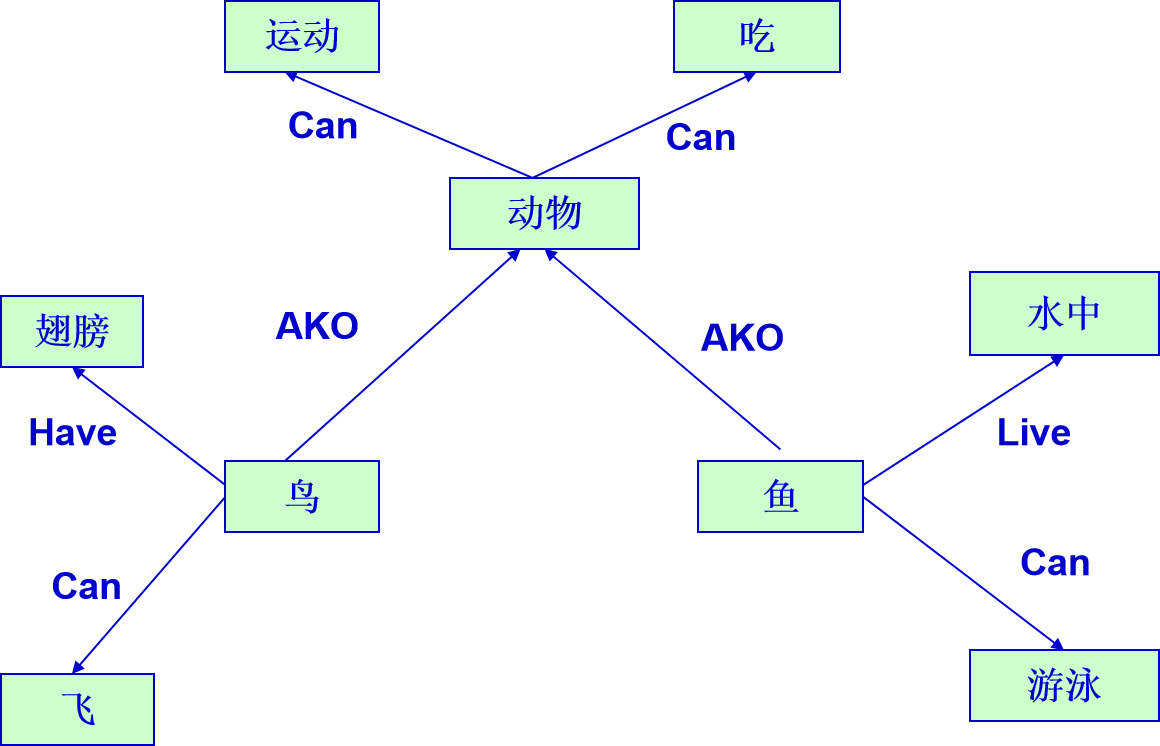
\includegraphics[width=0.45\textwidth]{eryuanguanxi2019112509.PNG}
\caption{例\ref{Chap2exam264}的语义网络}
\label{AI32fig09}
\end{figure}
%%%%%-------------------------------------
%%%%%--------------------------------
\begin{example}
用语义网络表示:
\begin{Verbatim}
        王强是理想公司的经理;
        理想公司在中关村;
        王强28岁.
\end{Verbatim}
%%%%%%%%%%%%%%%%%%%%%%%%%%%%%%
\begin{figure}[H]
\begin{center}
\begin{tikzpicture}[font={\sf \small}]
\def \smbwd{2cm}
\def \smbwe{4cm}
\thispagestyle{empty}
%定义流程图的具体形状
\node (qLPV) at (0,0) [draw, process,minimum width=\smbwd, minimum height=0.5cm] {王强};      % 王强
\node (UniSampling1)[draw, process,align=center,right=3cm of qLPV,yshift=-1.5cm] {28岁};      %28岁
\node (UniSampling2)[draw, process,align=center,right=3cm of qLPV,yshift=0cm] {经理};         %经理
\node (UniSampling3)[draw, process,align=center,right=3cm of qLPV,yshift=1.5cm] {理想公司};     %理想公司
\node (UniSampling4)[draw, process,align=center,right=3cm of UniSampling3,yshift=0cm] {中关村};%中关村
\draw[->] (qLPV.east)->(UniSampling1)node[left,yshift=0.15cm,xshift=-1.05cm,rotate=-25] {Age};
\draw[->] (qLPV.east)->(UniSampling2)node[left,yshift=0.25cm,xshift=-0.85cm] {Work-for};
\draw[->] (qLPV.east)->(UniSampling3)node[left,yshift=-0.25cm,xshift=-1.35cm,rotate=20] {Headship};
\draw[->] (UniSampling3)->(UniSampling4)node[left,yshift=0.25cm,xshift=-1.05cm] {Located-at};
\end{tikzpicture}
\caption{关于王强的语义网络}
\label{Wq2020021302}
\end{center}
\end{figure}
\end{example}
%%%%%%%%%%%%%%%%%%%%%%%%%%%%%%
%%%%%%%%%%%%%%%%%%%%%%%%%%%%%%%%例
\begin{example}\label{Chap2exam266}
李新的汽车的款式是“捷达”、银灰色.
王红的汽车的款式是“凯越”、红色.
李新和王红的汽车均属于具体概念,可增加“汽车” 这个抽象概念.
图\ref{AI32fig10}语义网络的基本网元.
\end{example}
%%%%%%%%%%%%%%%%%%%%%%%%%%%%%%%%
%%%%%-------------------------------------
\begin{figure}[htbp]
\centering
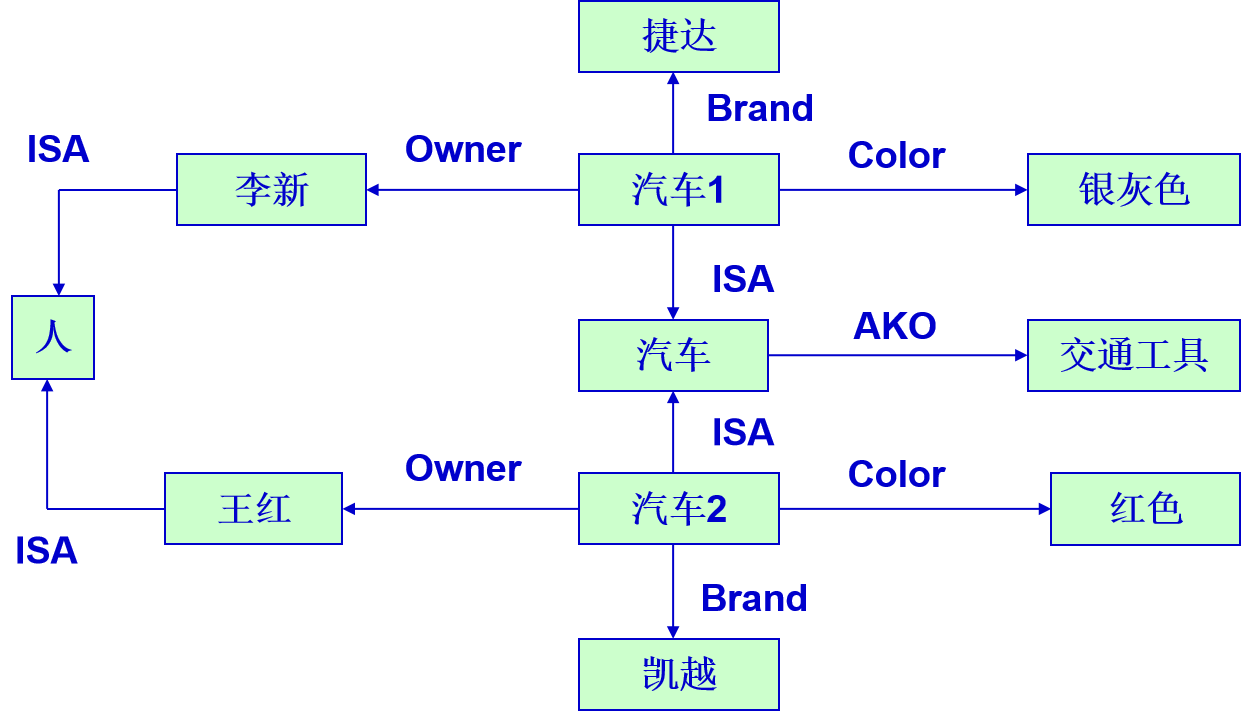
\includegraphics[width=0.45\textwidth]{tuli2019112510.PNG}
\caption{例\ref{Chap2exam266}的语义网络}
\label{AI32fig10}
\end{figure}
%%%%%-------------------------------------
%%%%%-----------------------------------------
\subsection{表示多元关系}
\begin{mydef}{多元关系}{1}
可用多元谓词$P(x_1, x_2,\cdots)$表示的关系, 其中, 个体$x_1, x_2,\cdots$为实体, 谓词$P$说明这些实体之间的关系.
\end{mydef}

用语义网络表示多元关系时, 可把它转化为一个或多个二员关系的组合, 然后再利用下一节讨论的合取关系的表示方法, 把这种多元关系表示出来.

多元关系的表示方法: 西蒙提出\uwave{增加情况和动作结点的描述方法}.
%%%%%%%%%%%%%%%%%%%%%%%%%%%%%%%%例
\begin{example}\label{Chap2exam268}
用语义网络表示: `\uwave{小燕子这只燕子从春天到秋天占有一个巢}".
\end{example}
需要设立一个\textbf{占有权结点}, 表示占有物和占有时间等.
%%%%%-------------------------------------
\begin{figure}[H]
\centering
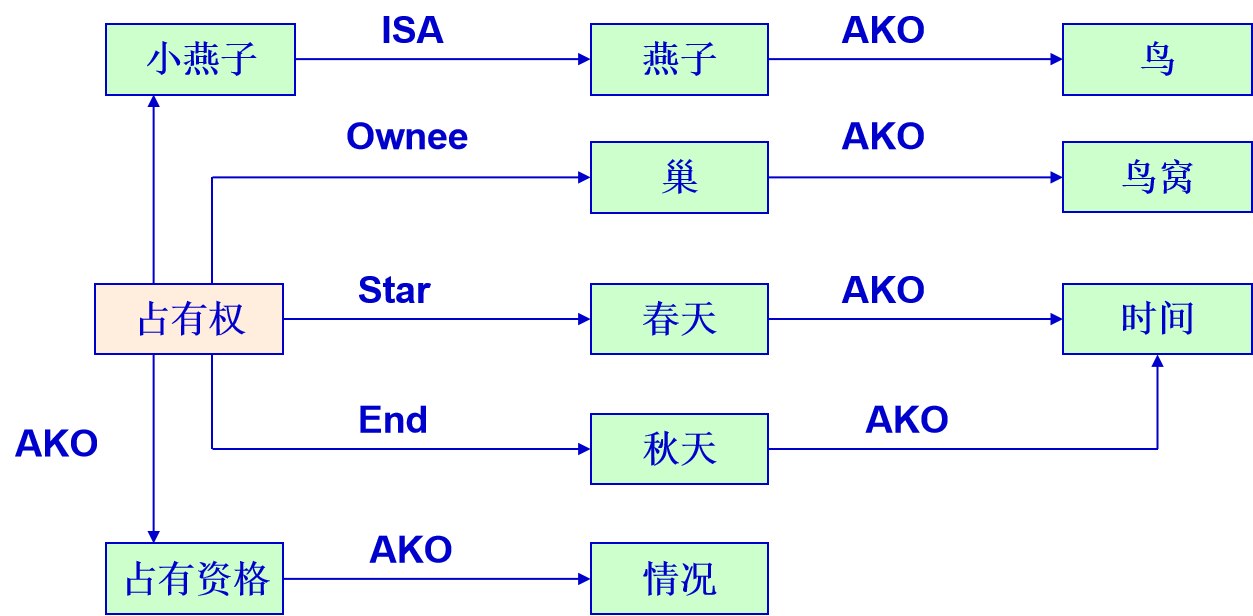
\includegraphics[width=0.45\textwidth]{tuli20191125101.PNG}
\caption{例\ref{Chap2exam268}的语义网络}
\label{AI32fig101}
\end{figure}
%%%%%-------------------------------------

对上述问题, 也可以把占有作为一种关系, 并用一条弧来表示, 但在这种表示方法下, 占有关系就无法表示了.
%%%%%-------------------------------------
\begin{figure}[H]
\centering
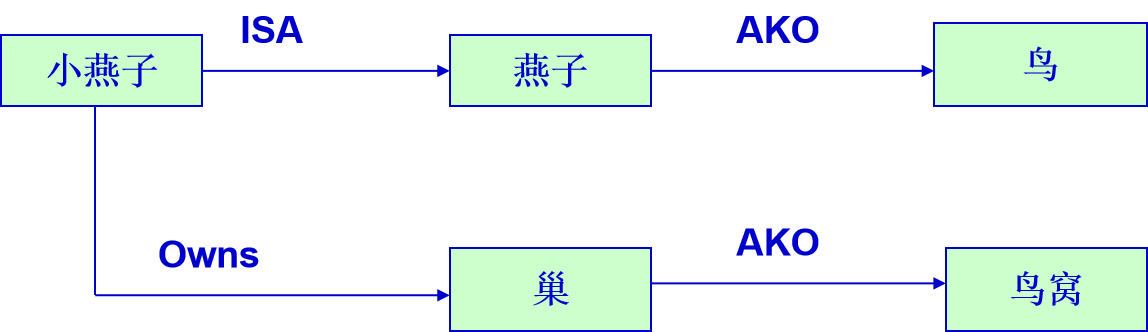
\includegraphics[width=0.45\textwidth]{tuli20191125102.PNG}
\caption{"小燕子这只燕子有一个巢"的语义网络}
\label{AI32fig102}
\end{figure}
%%%%%-------------------------------------
用语义网络表示事件或动作时, 需要设立一个事件或动作结点.

\textbf{动作结点}: 由一些向外引出的弧来指出动作的主体与客体.
%%%%%%%%%%%%%%%%%%%%%%%%%%%%%%%%例
\begin{example}\label{Chap2exam269}
用于语义网络表示: “常河给江涛一张磁盘作为礼物”.
\end{example}
%%%%%%%%%%%%%%%%%%%%%%%%%%%%%%%%

\textbf{事件结点}: 如上例用一个事件结点描述.

\textbf{表示方法}: 可通过增加合取结点和析取结点来实现.
%%%%%-------------------------------------
\begin{figure}[H]
\centering
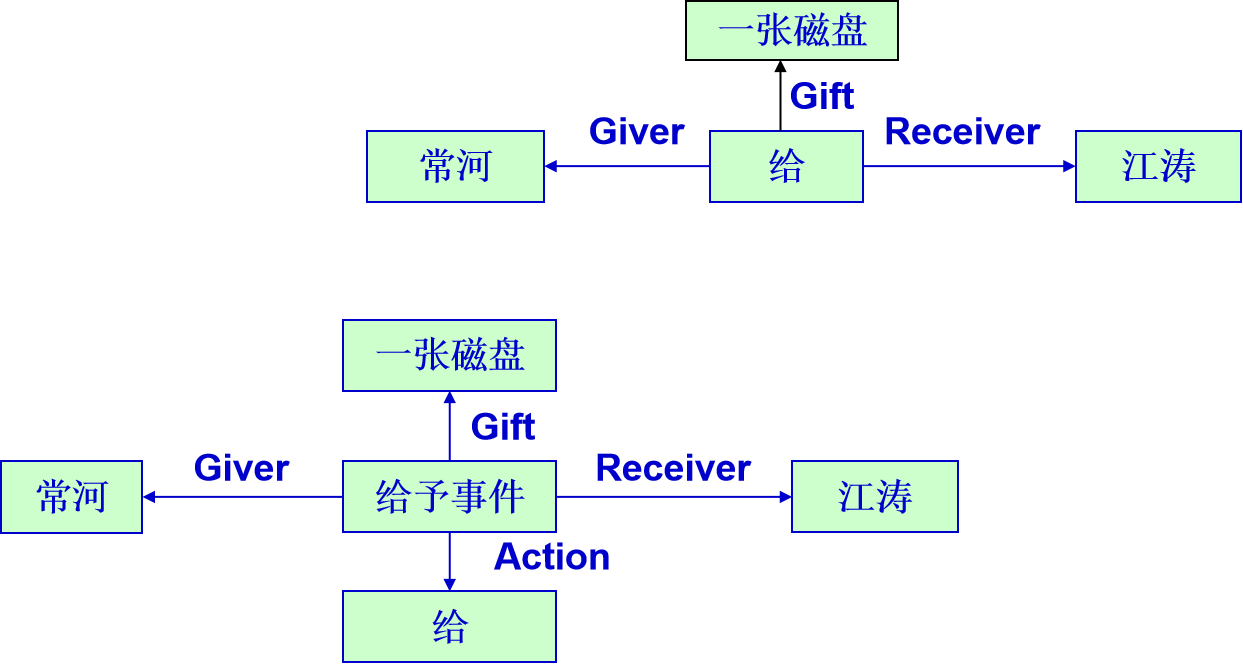
\includegraphics[width=0.5\textwidth]{tuli20191125103.PNG}
\vspace{-0.3cm}
\caption{例\ref{Chap2exam269}的语义网络}
\label{AI32fig103}
\end{figure}
%%%%%-------------------------------------
%%%%%%%%%%%%%%%%%%%%%%%%%%%%%%%%例
\begin{example}\label{Chap2exam270}
用语义网络表示如下事实: “参赛者有教师、有学生、有高、有低”.
\end{example}
%%%%%%%%%%%%%%%%%%%%%%%%%%%%%%%%
首先需要分析参赛者的不同情况, 可得到以下四种情况:
\begin{center}
\begin{Verbatim}
                A  教师、高;       B  教师、低.
                C  学生、高;       D  学生、低.
\end{Verbatim}
\end{center}
然后再按照他们的逻辑关系用语义网络表示出来.

可分为基本语义关系的否定和一般语义关系的否定. 基本语义关系的否定的表示, 可通过在有向弧上直接标注该基本语义关系的否定的方法来解决.
%%%%%-------------------------------------
\begin{figure}[H]
\centering
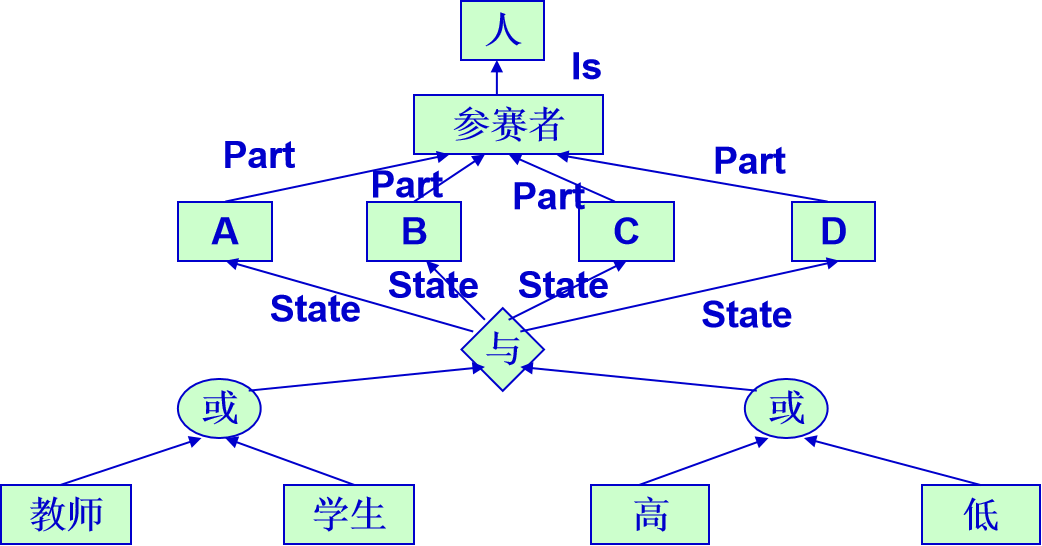
\includegraphics[width=0.46\textwidth]{tuli20191125104.PNG}
\caption{例\ref{Chap2exam270}的语义网络}
\label{AI32fig104}
\end{figure}
%%%%%-------------------------------------
%%%%%%%%%%%%%%%%%%%%%%%%%%%%%%%%例
\begin{example}
用语义网络表示: 书不在桌子上.
\end{example}
%%%%%%%%%%%%%%%%%%%%%%%%%%%%%%%%
采用在有向弧上直接标注该基本语义关系的否定的方法, 语义网络如图\ref{AI32fig00105}.
%%%%%%%%%%%%%%%%%%%%%%%%%%%%%%
\begin{figure}[H]
\begin{center}
\begin{tikzpicture}[font={\sf \small}]
\def \smbwd{2cm}
\def \smbwe{4cm}
\thispagestyle{empty}
%定义流程图的具体形状
\node (qLPV) at (0,0) [draw, process,minimum width=\smbwd, minimum height=0.5cm] {书};                  % 书
\node (UniSampling1)[draw, process,align=center,right=3.3cm of qLPV,yshift=0cm] {桌子};                 % 桌子
\draw[->] (qLPV.east)->(UniSampling1)node[left,yshift=0.25cm,rotate=0,xshift=-1.05cm] {$\neg$ Located-on};
\end{tikzpicture}
\caption{语义网络的基本网元}
\label{AI32fig00105}
\end{center}
\end{figure}
一般语义关系的否定的表示. 对一般语义关系的否定, 通常需要引进“非”节点来表示.
%%%%%%%%%%%%%%%%%%%%%%%%%%%%%%%%例
\begin{example}\label{Chap2exam271}
用语义网络表示:  常河没有给江涛一张磁盘.
\end{example}
%%%%%%%%%%%%%%%%%%%%%%%%%%%%%%%%
采用引进“非”节点的方法, 其语义网络如图\ref{AI32fig106}.
%%%%%-------------------------------------
%\begin{figure}[H]
%\centering
%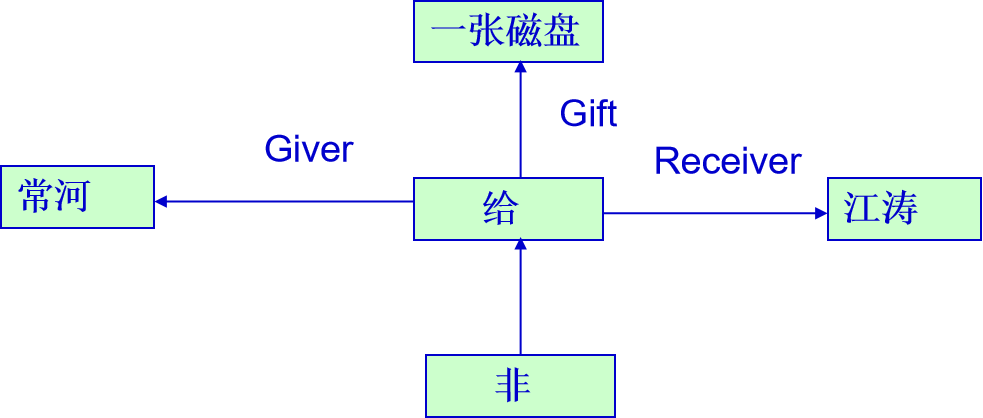
\includegraphics[width=0.76\textwidth]{tuli20191125106.PNG}
%\caption{语义网络的基本网元}
%\label{AI32fig106}
%\end{figure}
%%%%%%%%%%%%%%%%%%%%%%%%%%%%%%
\begin{figure}[H]
\begin{center}
\begin{tikzpicture}[font={\sf \small}]
\def \smbwd{2cm}
\def \smbwe{4cm}
\thispagestyle{empty}
%定义流程图的具体形状
\node (Gei) at (2,0) [draw, process,minimum width=\smbwd, minimum height=0.5cm] {给};   % 给
\node (jiangtao)[draw, process,align=center,right=3cm of Gei,yshift=0cm] {江涛};        %江涛
\draw[thick,->] (Gei.east)->(jiangtao) node[left,yshift=0.25cm,xshift=-1cm] {Receiver};
\node (Changhe)[draw, process,align=center,left=3cm of Gei,yshift=0cm] {常河};          %常河
\draw[thick,->](Gei.west)->(Changhe)node[right,yshift=0.25cm,xshift=1.5cm] {Giver};

\node (Cipan)[draw, process,align=center,above=1cm of Gei,yshift=0cm] {一张磁盘};       %磁盘
\draw[thick,->](Gei)->(Cipan)node[left,yshift=-0.75cm,xshift=0cm] {Gift};
\node (Fei)[draw, process,align=center,below=1cm of Gei,yshift=0cm] {非};              %非
\draw[thick,->](Fei)->(Gei.south)node[left,yshift=0.25cm,xshift=-1cm] {};
\end{tikzpicture}
\end{center}
\vspace{-0.3cm}
\caption{例\ref{Chap2exam271}的语义网络}
\label{AI32fig106}
\end{figure}
%%%%%-------------------------------------
%%%%%-----------------------------------------
\paragraph{蕴含的表示}
通过增加蕴含关系节点来实现.

在蕴含关系中, 有两条指向蕴含节点的弧, 一条代表前提条件, 标记为ANTE;另一条代表结论, 标记为CONSE.
\begin{example}\label{Chap2exam273}
 用语义网络表示如下知识:  “如果学校组织大学生机器人竞赛活动, 那么李强就参加比赛”.
\end{example}
该蕴含关系的语义网络如图\ref{AI32fig107},其中机器人竞赛的组织者是学校, 参赛对象是学生操纵的机器人, 而机器人只不过是一种智能机器.
%%%%%-------------------------------------
\begin{figure}[H]
\centering
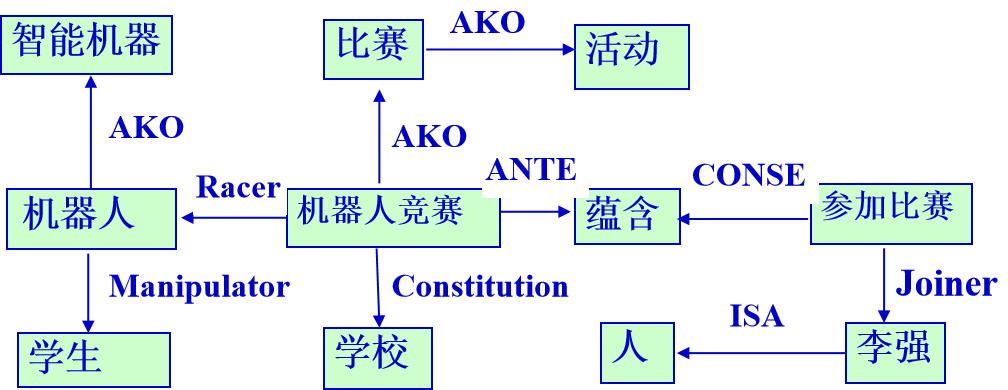
\includegraphics[width=0.6\textwidth]{tuli20191125107.PNG}
\caption{例\ref{Chap2exam273}的语义网络}
\label{AI32fig107}
\end{figure}
%%%%%-----------------------------------------
\subsection{存在和全称量词的表示}
\begin{center}
\begin{minipage}{0.9\textwidth}
\textcolor[rgb]{0,0,1}{\textbf{存在量词}}: 可直接用“ISA”、“AKO”等这样的语义关系来表示.

\textcolor[rgb]{0,0,1}{\textbf{全称量词}}: 可采用亨德里克提出的网络分区技术.

\textcolor[rgb]{0,0,1}{\textbf{基本思想}}: 把一个复杂命题划分为若干个子命题, 每个子命题用一个较简单的语义网络表示, 称为一个\textbf{子空间}, 多个子空间构成一个大空间.
每个子空间看作是大空间中的一个结点, 称作\textbf{超结点}. 空间可逐层嵌套, 子空间之间用弧互相连结.
\end{minipage}
\end{center}

%%%%%%%%%%%%%%%%%%%%%%%%%%%%%%%%例
\begin{example}\label{Chap2exam274}
用语义网络表示如下事实: “每个学生都学习了一门程序设计语言”.
\end{example}
%%%%%%%%%%%%%%%%%%%%%%%%%%%%%%%%
其语义网络如图\ref{AI32fig10007},
%%%%%-------------------------------------
\begin{figure}[H]
\centering
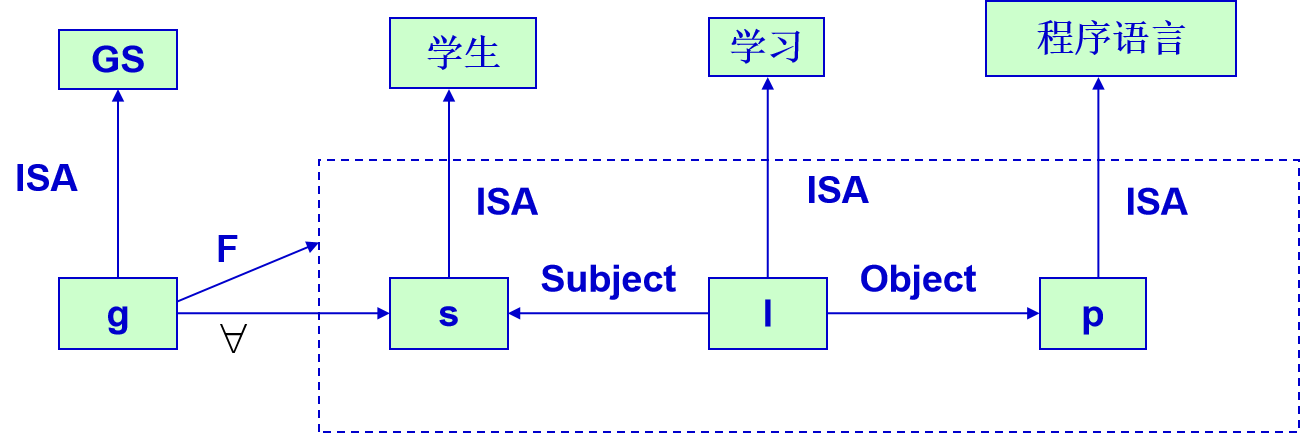
\includegraphics[width=0.6\textwidth]{tuli2019112910007.PNG}
\caption{例\ref{Chap2exam274}的语义网络}
\label{AI32fig10007}
\end{figure}
%%%%%-------------------------------------
\begin{flushleft}
      $GS$是一个概念结点, 它表示具有全称量化的一般事件.
      $g$是一个实例结点, 代表$GS$中的一个具体例子, 如上所提到的事实.
      $s$是一个全称变量, 表示任意一个学生.
      $I$是一个存在变量, 表示某一次学习.
      $P$是一个存在变量, 表示某一门程序设计语言.

      这样, $s,I,P$之间的语义联系就构成一个子空间, 它表示对每一个学生$s$, 都存在一个学习事件$I$ 和一门程序设计语言$P$.
\end{flushleft}
在从结点$g$引出的三条弧中, 弧“ISA”说明结点$g$是GS中一个实例; 弧“$F$”说明它所代表的子空间及其具体形式; 弧“$\forall$”说明它所代表的全称量词.
每一个全称量词都需要一条这样的弧, 子空间中有多少个全称量词, 就需要有多少条这样的弧.
%%%%%%%%%%%%%%%%%%%%%%%%%%%%%%%%例
\begin{example}\label{Chap2exam275}
用语义网络表示事实: “每个学生都学习了所有的程序设计课程”.
\end{example}
%%%%%%%%%%%%%%%%%%%%%%%%%%%%%%%%
其语义网络如图\ref{AI32fig1008}所示. 其中, 结点$g$有两条指向全称变量的弧.
%%%%%-------------------------------------
\begin{figure}[H]
\centering
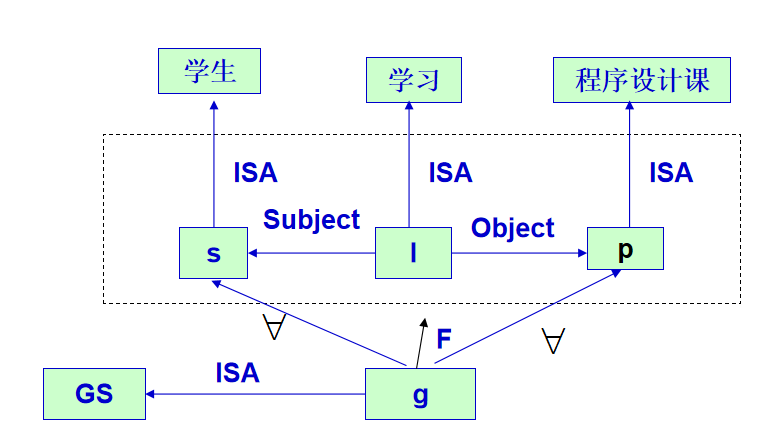
\includegraphics[width=0.5\textwidth]{tuli20191125108.PNG}
\caption{例\ref{Chap2exam275}的语义网络}
\label{AI32fig1008}
\end{figure}
%%%%%-------------------------------------

\begin{remark}
    在网络分区技术中, 要求$F$指向的子空间中的所有非全称变量结点都应该是存在量词约束的变量, 否则应放在子空间的外面.
\end{remark}

%%%%%%%%%%%%%%%%%%%%%%%%%%%%%%%%例
\begin{example}\label{Chap2exam276}
用语义网络表示事实: “每个学生都学习了C++语言”.
\end{example}
%%%%%%%%%%%%%%%%%%%%%%%%%%%%%%%%
其语义网络如图\ref{AI32fig109}所示. 结点“C++语言”代表一门具体的程序设计语言, 是结点“程序语言”的一个实例, 故被放到$F$所指的子空间的外边.
%%%%%-------------------------------------
\begin{figure}[H]
\centering
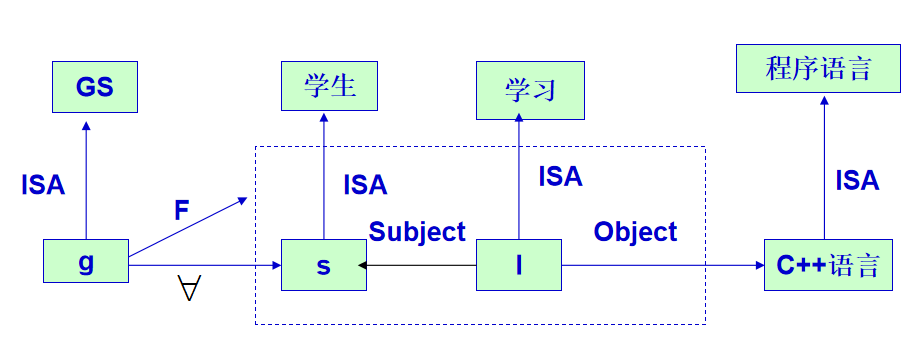
\includegraphics[width=0.56\textwidth]{tuli20191125109.PNG}
\caption{例\ref{Chap2exam276}的语义网络}
\label{AI32fig109}
\end{figure}
%%%%%-----------------------------------------
\subsection{语义网络的推理过程}
用语义网络表示知识的问题求解系统主要由两大部分所组成, 一部分是由语义网络构成的知识库, 另一部分是用于问题求解的推理机构.
语义网络的推理过程主要有两种, 一种是\uwave{继承}, 另一种是\uwave{匹配}.
%%%%%%%%%%%%%%%%%%%%%%%%%%%%%%%%
\subsection{继承}
%%%%------------------------------------
\begin{mydef}{继承}{1}
指把对事物的描述从\uwave{抽象结点传递到实例结点}. 通过继承可以得到所需结点的一些属性值, 它通常是沿着ISA和AKO等继承弧进行的.
\end{mydef}
%%%%%%%%%%%%%%%%%%%%%%%%%%%%%%%%
\paragraph{继承的一般过程} 继承是在结点上用弧表示彼此的连接、从属和属性关系,  从上一节点得到需要的属性.

(1) 建立一个结点表, 用来存放待求解结点和所有以ISA、AKO等继承弧与此结点相连的那些结点. 初始情况下, 表中只有待求解结点.

(2) 检查表中的第一个结点是否是有继承弧. 如果有,就把该弧所指的所有结点放入结点表的末尾, 记录这些结点的所有属性, 并从结点表中删除第一个结点. 如果没有继承弧, 仅从结点表中删除第一个结点.

(3) 重复(2), 直到结点表为空. 此时, 记录下来的所有属性都是待求解结点继承来的属性.
%%%%%%%%%%%%%%%%%%%%%%%%%%%%%%%%例
\begin{example}
  在图\ref{AI32fig09}所示的语义网络中, 通过继承关系可以得到“鸟”具有: 会吃、能运动的属性.
\end{example}
%%%%%-----------------------------------------
\subsection{匹配}
\begin{mydef}{匹配}{1}
    指在知识库的语义网络中寻找与待求解问题相符的语义网络模式.
\end{mydef}匹配的主要过程:

    (1) 根据待求解问题的要求构造一个网络片断, 该网络片断中有些结点或弧的标识是空的, 称为\textbf{询问处}, 它反映的是待求解的问题.

    (2) 根据该语义片断到知识库中去寻找所需要的信息.

    (3) 当待求解问题的网络片断与知识库中的某语义网络片断相匹配时, 则与询问处相匹配的事实就是问题的解.
%%%%%%%%%%%%%%%%%%%%%%%%%%%%%%%%例
\begin{example}\label{Chap2exam278}
    假设例\ref{Wq2020021302}的语义网络已在知识库中, 问王强在哪个公司工作.
\end{example}
%%%%%%%%%%%%%%%%%%%%%%%%%%%%%%%%

根据这个问题的要求, 可构造如下语义网络片断.
%%%%%%%%%%%%%%%%%%%%%%%%%%%%%%
\begin{figure}[H]
\begin{center}
\begin{tikzpicture}[font={\sf \small}]
\def \smbwd{2cm}
\def \smbwe{4cm}
\thispagestyle{empty}
%定义流程图的具体形状
\node (qLPV) at (0,0) [draw, process,minimum width=\smbwd, minimum height=0.5cm] {?};      % ?
\node (UniSampling1)[draw, process,align=center,right=3cm of qLPV,yshift=0cm] {王强};      % 王强
\draw[->] (qLPV.east)->(UniSampling1)node[left,yshift=0.25cm,xshift=-1.05cm] {Work for};
\end{tikzpicture}
\caption{例\ref{Chap2exam278}的语义网络}
\label{AI32fig105}
\end{center}
\end{figure}
当用该语义网络片段与图\ref{Wq2020021302}所示的语义网络进行匹配时, 由“工作在”弧所指的结点可知, 职员王强工作在“理想公司”, 这就得到了问题的答案.
若还想知道职员王强的其它情况, 则可在语义网络中增加相应的空结点.
%%%%%-----------------------------------------
\subsection{语义网络表示法的特征}
    主要优点:
\begin{itemize}
    \item \uwave{结构性} 把事物的属性以及事物间的各种语义联系显式地表示出来, 是一种结构化的知识表示方法. 在这种方法中, 下层结点可以继承、新增、变异上层结点的属性.
    \item \uwave{联想性} 本来是作为人类联想记忆模型提出来的, 它着重强调事物间的语义联系, 体现了人类的联想思维过程.
    \item \uwave{自索引性} 把各接点之间的联系以明确、简洁的方式表示出来, 通过与某一结点连结的弧可以很容易的找出与该结点有关的信息, 而不必查找整个知识库. 这种自索引能力有效的避免搜索时所遇到的组合爆炸问题.
    \item \uwave{自然性} 这种带有标识的有向图, 可比较直观地把知识表示出来, 符合人们表达事物间关系的习惯, 并且与自然语言语义网络之间的转换也比较容易实现.
\end{itemize}
主要缺点:
\begin{itemize}
    \item \uwave{非严格性} 没有象谓词那样严格的形式表示体系, 一个给定语义网络的含义完全依赖于处理程序对它所进行的解释, 通过语义网络所实现的推理不能保证其正确性.
    \item \uwave{复杂性} 语义网络表示知识的手段是多种多样的, 这虽然对其表示带来了灵活性, 但同时也由于表示形式的不一致, 使得它的处理增加了复杂性.
\end{itemize}
%%%%%-----------------------------------------
\section{框架表示法}
\begin{mydef}{框架表示法}{1}
    在框架理论的基础上发展起来的一种结构化知识表示方法.
\end{mydef}
%2.5.1 框架理论
%
%2.5.2 框架和实例框架
%
%2.5.3 框架系统
%
%2.5.4 框架系统的问题求解过程
%
%2.5.5 框架表示法的特征
%%%%%-----------------------------------------
\subsection{框架理论}
    框架理论是明斯基于1975年作为理解视觉、自然语言对话及其它复杂行为基础的智能行为提出来的一种方法.
它认为人们对现实世界中各种事物的认识都是以一种类似于框架的结构存储在记忆中的, 当遇到一个新事物时, 就从记忆中找出一个合适的框架, 并根据新的情况对其细节加以修改和补充, 从而形成对这个新事物的认识.

\begin{example}
    对饭店、教室等的认识.
\begin{itemize}
    \item \textbf{框架}: 是人们认识事物的一种通用的数据结构形式. 即当新情况发生时, 人们只要把新的数据加入到该通用数据结构中便可形成一个具体的实体(类), 这样的通用数据结构就称为框架.
    \item \textbf{实例框架}: 对于一个框架, 当人们把观察或认识到的具体细节填入后, 就得到了该框架的一个具体实例, 框架的这种具体实例被称为实例框架.
    \item \textbf{框架系统}: 在框架理论中, 框架是知识的基本单位, 把一组有关的框架连结起来便可形成一个框架系统.
    \item \textbf{框架系统推理}: 由框架之间的协调来完成.
\end{itemize}
\end{example}
%%%%%-----------------------------------------
\subsection{框架结构和框架表示}
%%%%%%%%%%%%%%%%%%%%%%%%%%%%%%%%例
\begin{example}
一个直接描述硕士生有关情况的框架.
\end{example}
%%%%%%%%%%%%%%%%%%%%%%%%%%%%%%%%原文引用
\begin{Verbatim}
Frame <MASTER>
    Name: Unit(Last-name, First-name)
    Sex: Area(male, female)
              Default:  male
    Age: Unit(Years)
    Major: Unit(Major)
    Field: Unit(Field)
    Advisor: Unit(Last-name, First-name)
    Project : Area(National, Provincial, Other)
                     Default: National
    Paper: Area(SCI, EI, Core, General)
                  Default: Core
    Address: <S-Address>
    Telephone: Home  Unit(Number)
     Mobile  Unit(Number)
\end{Verbatim}

%%%%%-----------------------------------------
\paragraph{框架的基本结构}
%%%%%%%%%%%%%%%%%%%%%%%%%%%%%%%%原文引用
\begin{Verbatim}
<框架名>
槽名1:   侧面名11       值111, 值112, ……
                 侧面名12       值121, 值122, ……
                     :
槽名2:   侧面名21       值211, 值212, ……
                 侧面名22       值221, 值222, ……
                      :
    :
    :
槽名n:   侧面名n1       值n11, 值n12, ……
                 侧面名n2       值n21, 值n22, ……
                      :
                 侧面名nm     值nm1, 值nm2, ……
\end{Verbatim}

%%%%%-----------------------------------------
\paragraph{学生框架}
%%%%%%%%%%%%%%%%%%%%%%%%%%%%%%%%原文引用
\begin{Verbatim}
Frame <Student>
    Name: Unit(Last-name, First-name)
    Sex: Area(male, female)
              Default: male
    Age: Unit(Years)
              If-Needed: Ask-Age
    Address: < S-Address>
    Telephone: Home  Unit(Number)
                        Mobile  Unit(Number)
                        If-Needed: Ask-Telephone
\end{Verbatim}
%%%%%-----------------------------------------
\paragraph{硕士生框架}
%%%%%%%%%%%%%%%%%%%%%%%%%%%%%%%%原文引用
\begin{Verbatim}
Frame <Master>
    AKO: Student
    Major: Unit(Major)
                If-Needed: Ask- Major
                       If-Added: Check-Major
    Field: Unit(Direction-Name)
                If- Needed: Ask - Field
    Advisor: Unit(Last-name, First-name)
                     If-Needed: Ask-Visor
    Project : Area(National, Provincial, Other)
                    Default: National
    Paper: Area(SCI, EI, Core, General)
                  Default: Core
\end{Verbatim}
在Master框架中, 用到了一个系统预定义槽名AKO. 所谓\textbf{系统预定义槽名}, 是指框架表示法中事先定义好的可公用的一些标准槽名. AKO与其在语义网络中的含义相似, 其直观含义为“是一种”.
当AKO作为下层框架的槽名时, 其槽值为上层框架的框架名, 表示该下层框架所描述的事物比其上层框架更具体. 并且, 由AKO所联系的框架之间具有属性的继承关系.

框架的继承技术, 通常由框架中设置的3个侧面: Default、If- Needed、If-Added所提供的缺省推理功能来组合实现.

\textbf{Default}: 该侧面的作用是为相应槽提供缺省值. 当其所在槽没有填入槽值时, 系统就以此侧面值作为该槽的默认值.
\begin{example}
  Paper槽的默认值为Core.
\end{example}

\textbf{If- Needed}: 该侧面的作用是提供一个为相应槽赋值的过程. 当某个槽不能提供统一的缺省值时, 可在该槽增加一个If-Needed侧面, 系统通过调用该侧面提供的过程, 产生相应的属性值.
\begin{example}
  Age 槽、Telephone槽等.
\end{example}

\textbf{If-Added}: 该侧面的作用是提供一个因相应槽值变化而引起的后继处理过程. 当某个槽的槽值变化会影响到一些相关槽时, 需要在该槽增加一个If-Added侧面, 系统通过调用该侧面提供的过程去完成对其相关槽的后继处理.
\begin{example}
  Major槽, 由于专业的变化, 可能会引起Field和Advisor的变化, 因此需要调用If-Added侧面提供的Check-Major过程进行后继处理.
\end{example}
%%%%%-----------------------------------------
\paragraph{实例框架}
\begin{example}
  假设有杨叶和柳青2个硕士生, 当把他们的具体情况分别添入Master框架后, 可得实例框架Master-1和Master-2.
\end{example}
这2个实例框架可表示如下:

硕士生-1框架:
%%%%%%%%%%%%%%%%%%%%%%%%%%%%%%%%原文引用
\begin{Verbatim}
Frame <Master-1>
    ISA: Master
    Name: Yang Ye
    Sex:  female
    Major: Computer
    Field: Web-Intelligence
    Advisor: Lin Hai
    Project : Provincial
\end{Verbatim}

硕士生-2框架:
%%%%%%%%%%%%%%%%%%%%%%%%%%%%%%%%原文引用
\begin{Verbatim}
Frame <Master-2>
    ISA: Master
    Name: Liu Qing
    Age: 22
    Major: Computer
    Advisor: Lin Hai
    Paper:  EI
\end{Verbatim}
在这2个实例框架中, 我们又用到了一个系统预定以槽名ISA. 该预定义槽名与语义网络中的ISA弧的语义相似, 其直观含义为“是一个”, 表示一个事物是另一个事物的一个具体实例, 用来描述一个具体事物与其抽象概念间的实例关系.
\begin{example}
  Master-1和Master-2是2个具体的Master.
\end{example}
%%%%%-----------------------------------------
\paragraph{框架系统的基本结构}
当知识比较复杂时, 往往需要通过诸框架之间的横向或纵向联系形成一种框架系统.
%%%%%-----------------------------------------
\subparagraph{框架之间的纵向联系}
是指那种具有继承关系的上下层框架之间的联系.
\begin{example}
  在图\ref{AI32fig11}中, 学生可按照接受教育的层次分为本科生、硕士生和博士生. 每类学生又可按照所学专业的不同, 分为不同专业的学生等.
\end{example}

框架之间的纵向联系是通过预定以槽名AKO和ISA等来实现的.
\begin{example}
  前面的例子, AKO实现了Student框架与Master框架之间的纵向联系, ISA实现了Master框架与Master-1实例框架之间的联系.
\end{example}
\subparagraph{框架之间的横向联系}
是指那种以另外一个框架名作为一个槽的槽值或侧面值所建立起来的框架之间的联系. 如下图给出的框架系统中, Student框架与S-Addre框架之间就是一种横向联系(图\ref{AI32fig11}).
%%%%%-------------------------------------
\begin{figure}[H]
\centering
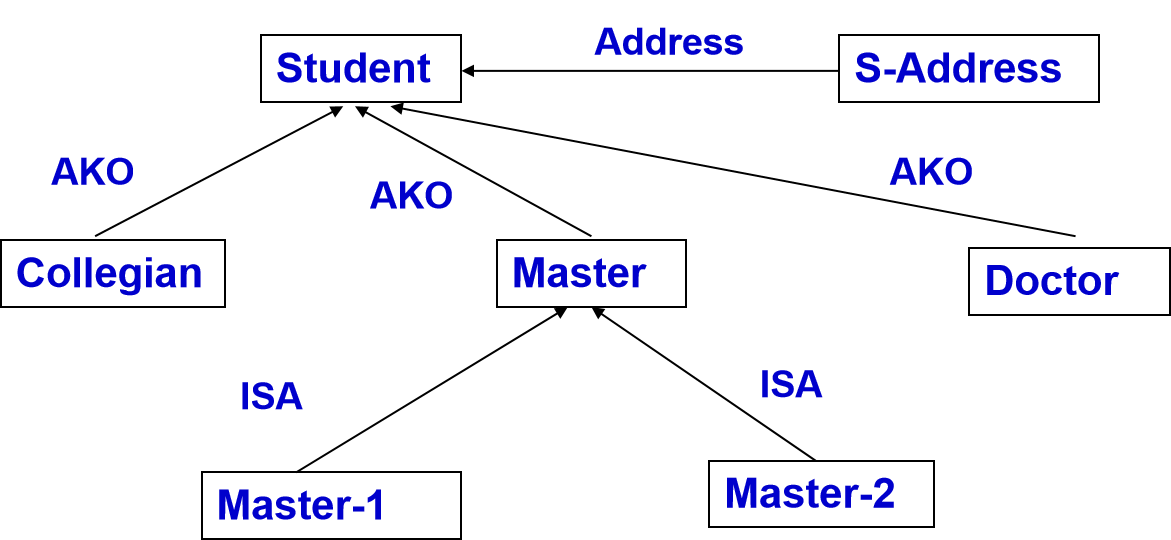
\includegraphics[width=0.6\textwidth]{kuangjia2019112511.PNG}
\caption{框架系统的基本结构}
\label{AI32fig11}
\end{figure}
%%%%%-----------------------------------------
\paragraph{基本过程}
在框架系统中, 问题求解主要是通过对框架的继承、匹配与填槽来实现的. 求解问题分为如下三步:

1) 把该问题用框架表示出来.

2) 利用框架之间的继承关系, 把它与知识库中的已有框架进行匹配, 找出一个或多个候选框架, 并在这些候选框架引导下进一步获取附加信息, 填充尽量多的槽值, 以建立一个描述当前情况的实例.

3) 再用某种评价方法对候选框架进行评价, 以决定是否接收该框架.
%%%%%-----------------------------------------
\paragraph{特性继承}
特性继承过程
\begin{itemize}
\item  特性继承主要是通过ISA、AKO链来实现的. 当需要查询某一事物的某个属性, 且描述该事物的框架为提供其属性值时, 系统就沿ISA和AKO链追溯到具有相同槽的类或超类框架.
\item  如果该槽提供有Default侧面值, 就继承该默认值作为查询结果返回.
\item  如果该槽提供有If-Needed侧面供继承, 则执行If-Needed操作, 去产生一个值作为查询结果.
\item  如果对某个事物的某一属性进行了赋值或修改操作, 则系统会自动沿ISA和AKO链追溯到具有相应的类或超类框架, 只要发现类或超类框架中的同名槽具有If-Added侧面, 就执行If-Added操作, 作相应的后继处理.
\end{itemize}
%%%%%-----------------------------------------
\paragraph{If-Needed与If-Added过程的区别}
它们的主要区别在于激活时机和操作目的不同.
\begin{itemize}
\item If-Needed操作是在系统试图查询某个事物框架中未记载的属性值时激活, 并根据查询需求, 被动地即时产生所需要的属性值;
\item If-Added操作是在系统对某个事务框架的属性作赋值或修改工作后激活, 目的在于通过规定的后继处理, 主动做好配套操作, 以消除可能存在的不一致问题.
\end{itemize}
\begin{example}
以前面的学生框架为例
\begin{itemize}
\item 若要查询Master-1的Sex, 则可直接回答;但要查询Master-2的Sex, 则需要沿ISA链和AKO链到Student框架取其默认值male.
\item 若要查询Master-2的Field, 需要沿ISA链到Master框架, 执行Field槽If-Needed侧面的Ask-Field操作, 即时产生一个值, 假设产生的值是Data-Mining, 则表示Master-2的研究方向为数据挖掘.
\item 如果要修改Master-2的Major, 需要沿ISA链到Master框架, 执行Major槽If-Added侧面的Check-Major操作, 对Field、Advisor进行修改, 以保持知识的一致性.
\end{itemize}
\end{example}
%%%%%-----------------------------------------
\paragraph{匹配和填槽}
框架的匹配实际上是通过对相应槽的槽名和槽值逐个进行比较, 并利用继承关系来实现的.
\begin{example}
假设前面讨论的学生框架系统已建立在知识库中, 若要求从知识库中找出一个满足如下条件的硕士生:
\begin{center}
  male, Age<25>, Major为Computer, Project为National
\end{center}
把这些条件用框架表示出来, 就可得到如下的初始问题框架:
\begin{Verbatim}
    Frame: Master-x
        Name:
        Age: Years <25>
        Sex: male
        Major: Computer
        Projec: National
\end{Verbatim}
\end{example}
用此框架和知识库中的框架匹配, 显然“Master -2”框架可以匹配. 因为Age、Sex 、Major槽都符合要求, Project槽虽然没有给出, 但由继承性可知它取默认值National, 完全符合初始问题框架Master-x的要求, 所以要找的学生有可能是Liu Qing.
%%%%%-----------------------------------------
\subsection{框架表示法的特征}
框架表示法的优点
\begin{itemize}
\item 结构性: 最突出特点是善于表示结构性知识, 它能够把知识的内部结构关系以及知识间的特殊联系表示出来.
\item 深层性:  框架表示法不仅可以从多个方面、多重属性表示知识, 而且还可以通过ISA、AKO等槽以嵌套结构分层地对知识进行表示, 因此能用来表达事物间复杂的深层联系.
\item 继承性: 在框架系统中, 下层框架可以继承上层框架的槽值, 也可以进行补充和修改, 这样既减少知识冗余, 又较好地保证了知识的一致性.
\item 自然性: 框架能把与谋个实体或实体集相关特性都集中在一起, 从而高度模拟了人脑对实体多方面、多层次的存储结构, 直观自然, 易于理解.
\end{itemize}

\indent\textbf{框架表示法的不足}
\begin{itemize}
\item 缺乏框架的形式理论: 至今, 还没有建立框架的形式理论, 其推理和一致性检查机制并非基于良好定义的语义.
\item 缺乏过程性知识表示: 框架系统不便于表示过程性知识, 缺乏如何使用框架中知识的描述能力. 框架推理过程需要用到一些与领域无关的推理规则, 而这些规则在框架系统中又很难表达.
\item 清晰性难以保证: 由于各框架本身的数据结构不一定相同, 从而框架系统的清晰性很难保证.
\end{itemize}
%%%%%-----------------------------------------
\section{过程表示法}
过程性知识表示是将有关某一问题领域的知识, 连同如何使用这些知识的方法, 均隐式地表示为一个求解问题的过程.
%
%2.6.1 知识表示方法
%
%2.6.2 过程表示的问题求解过程
%
%2.6.3过程表示的特性

过程表示没有固定的表示形式, 如何描述知识完全取决于具体问题. 以过程规则表示形式为例, 一个过程规则由以下4部分组成:

(1) 激发条件
\begin{itemize}
\item 激发条件由推理方向和调用模式两部分组成.
\item 推理方向用于指出推理是正向推理(FR)还是反向推理(BR).
\item 正向推理, 只有当综合数据库中的已有事实可以与其“调用模式”匹配时, 该过程规则才能被激活;
\item 反向推理, 只有当“调用模式”与查询目标或子目标匹配时才能将该过程规则激活.
\end{itemize}

(2) 演绎操作: 演绎操作由一系列的子目标构成. 当前面的激发条件满足时, 将执行这里列出的演绎操作.

(3) 状态转换: 状态转换槽的作用是来完成对综合数据库的增、删、改操作.

(4) 返回: 过程规则的最后一个语句使返回语句, 用于指出将控制权返回到调用该过程规则的上一级过程规则那里去.
%%%%%---------------------------------------------
\begin{example}
下面给出一个关于同学问题的过程表示.

     设有如下知识:

         “如果$x$与$y$是同班同学, 且$z$是$x$的老师,  则$z$也是$y$的老师”

    其过程规则表示为:

             BR(Teacher, ?z, ?y)         (需求解的问题)

             GOAL(Classmate, ?$x, y$)   (求$y$的同班同学是谁)

             GOAL(Teacher, $z, x$)       (已知$z$是$x$的老师)

             INSERT(Teacher,  $z, y$)     (对数据库的插入操作)

             RETURN

其中: BR是逆向推理标志;

     GOAL表示求解子目标, 即进行过程调用;

     INSERT表示对数据库进行插入操作;

     RETURN作为结束标志;

     带“?”的变量表示其值将在该过程中求得.
\end{example}
问题求解的基本过程:

每当有一个新的目标时, 就从可以匹配的过程规则中选择一个执行之. 在该规则的执行过程中可能会产生新的目标, 此时就调用相应的过程规则并执行它. 反复进行这一过程, 直至执行到RETURN语句.
只要碰到 RETURN语句, 就将调用返回当前过程的上一级过程规则, 并依次逐级返回.
如果某过程规则运行失败, 就另选择一个同层的可匹配过程规则执行, 如果不存在这样的过程规则, 则返回失败标志, 并将控制权移交给上一级过程规则.

%%%%%---------------------------------------------
\begin{example}
设综合数据库中有以下已知事实:
\begin{center}
(Classmate,杨叶,柳青)

(Teacher,林海,杨叶)
\end{center}
已知杨叶与柳青是同班同学, 林海是杨叶的老师.

假设需要求解的问题是: 找出两个人$w$及$v$, 其中$w$是$v$的老师.

该问题可表示为: GOAL(Teacher, ?w, ?v).
\end{example}
%%%%-----------------------------------
\begin{answer}
     (1) 在过程规则库中找出对于问题GOAL(Teacher,?w, ?v), 其激发条件可以满足的过程规则. 显然, BR(Teacher,  z, y)经如下变量代换$w/z,  v/y$后可以匹配, 因此选用该过程规则.

(2) 执行该过程规则中的第一个语句GOAL(Classmate, ?x, y). 此时, 其中的$y$已被$v$代换. 经与已知事实(Classmate,杨叶,柳青)匹配, 分别求得了变量$x$及$v$的值, 即
\begin{center}
  $x$=杨叶,$v$=柳青
\end{center}

(3) 执行该过程规则中的第二个语句GOAL(Teacher, z, x). 此时, $x$的值已经知道, $z$已被$w$代换. 经与已知事实(Teacher, 林海 ,杨叶)匹配, 求得了变量$w$的值, 即
\begin{center}
  $w$=林海
\end{center}

(4) 执行该过程规则中的第三个语句INSERT(Teacher, z, y), 此时, $z$与$y$的值均以知道, 分别是林海和杨叶, 因此这时插入数据库的事实是:
\begin{center}
    (Teacher,林海,   杨叶)
\end{center}
这表明“林海也是杨叶的老师”, 求得了问题的解.
\end{answer}
%%%%%-----------------------------------------
\subsection{过程表示的主要优缺点}
\begin{itemize}
\item  表示效率高.
\item  过程表示法是用程序来表示知识的, 而程序能准确的表明先做什么, 后作什么以及怎样做, 并直接嵌入一些启发式的控制信息, 因此, 可以避免选择及匹配那些无关的知识, 也不需要跟踪那些不必要的路径, 从而提高了系统的运行效率.
\item  控制系统容易实现.
\item  由于控制性质是已嵌入到程序中, 因而控制系统就比较容易设计.
\end{itemize}

主要缺点: 不易修改及添加新知识, 而且当对某一过程进行修改时, 又可能影响到其它过程, 对系统的维护带来不便.
%%%%%-----------------------------------------
\section{问题规约法}
%%%%%-----------------------------------------
\section{模糊认知图}
\begin{mydef}{模糊认知图}{1}
模糊认知图(Fuzzy Cognitive Map, FCM, 1986)是Kosko融合Zadeh的模糊集理论和Axelrod的认知图理论提出的, 将概念间的三值关系\{-1,0,1\}扩展成为区间[-1,1]上的模糊关系发展而来.
\end{mydef}
FCM 的概念值和弧的权值都可以为模糊值, 是一种软计算方法, 它是模糊逻辑和神经网络结合的产物, FCM的知识表示和推理能力更强.
模糊认知图是个有向图, 它将模糊反馈动力系统中的概念及概念间的关系通过弧线连接起来, 强调“结构就是含义”.

将模糊反馈动力系统中的因果事件、参与值、目标与趋势等通过各概念问的弧线连接起来的图结构, 节点是概念、实体等, 弧表示概念或实体间的因果关系, 在结构上可以看作是面向对象的单层带反馈的神经网络. 与神经网络不同的是, 模糊认知图的每个节点与弧都有很强的语义, 从而使整个图都呈现很强的语义. 它支持专家先验知识及因果关系的表示与推理, 这些都蕴涵在概念节点及概念节点间的关系中, 并且可以通过概念间的关系来表示模糊推理, 由整个图中各概念节点的相互作用来模拟系统的动态行为, 是一种无监督模型. 其概念可以是系统的事件、目标、感情及趋势等;概念值为模糊值, 也可以是二值, 反映该节点对某概念以某种程度发生或表示概念状态是关还是开. 概念节点的输出与概念节点自身的状态水平和外部因果联系的强度有关. 模糊认知图的有限输入状态可在虚拟空间中开辟一条通路, 简单模糊认知图的通路可能终止于固定点或极限环, 而对于具有反馈的复杂模糊认知图可能终止于“混沌”的奇异吸引子.
%%%%%-------------------------------------------------------------------
\section{作业}

%%%%%------------------------------------------
\begin{think}
请用语义网络表示如下知识: 高老师从3月到7月给计算机系的学生讲“计算机网络”课.
\end{think}

%%%%%------------------------------------------
\begin{observe}
用谓词逻辑知识表示方法表示如下知识:

(1) 有人喜欢梅花, 有人喜欢菊花, 有人既喜欢梅花又喜欢菊花.

(2) 不是每个计算机系的学生都喜欢在计算机上编程序.
\end{observe}

%%%%%------------------------------------------
\begin{think}
  人工智能对知识表示有什么要求?
\end{think}

%%%%%------------------------------------------
\begin{think}
用一阶谓词逻辑表示下面的句子: a)并不是所有的学生选修了历史和生物.  b)历史考试中只有一个学生不及格.
c)只有一个学生历史和生物考试都不及格. d)历史考试的最高分比生物考试的最高分要高.
\end{think}

%%%%%------------------------------------------
\begin{think}
语义网络示例如图\ref{YUYINETlizi01}, 给出其描述.
\begin{figure}[H]
\centering
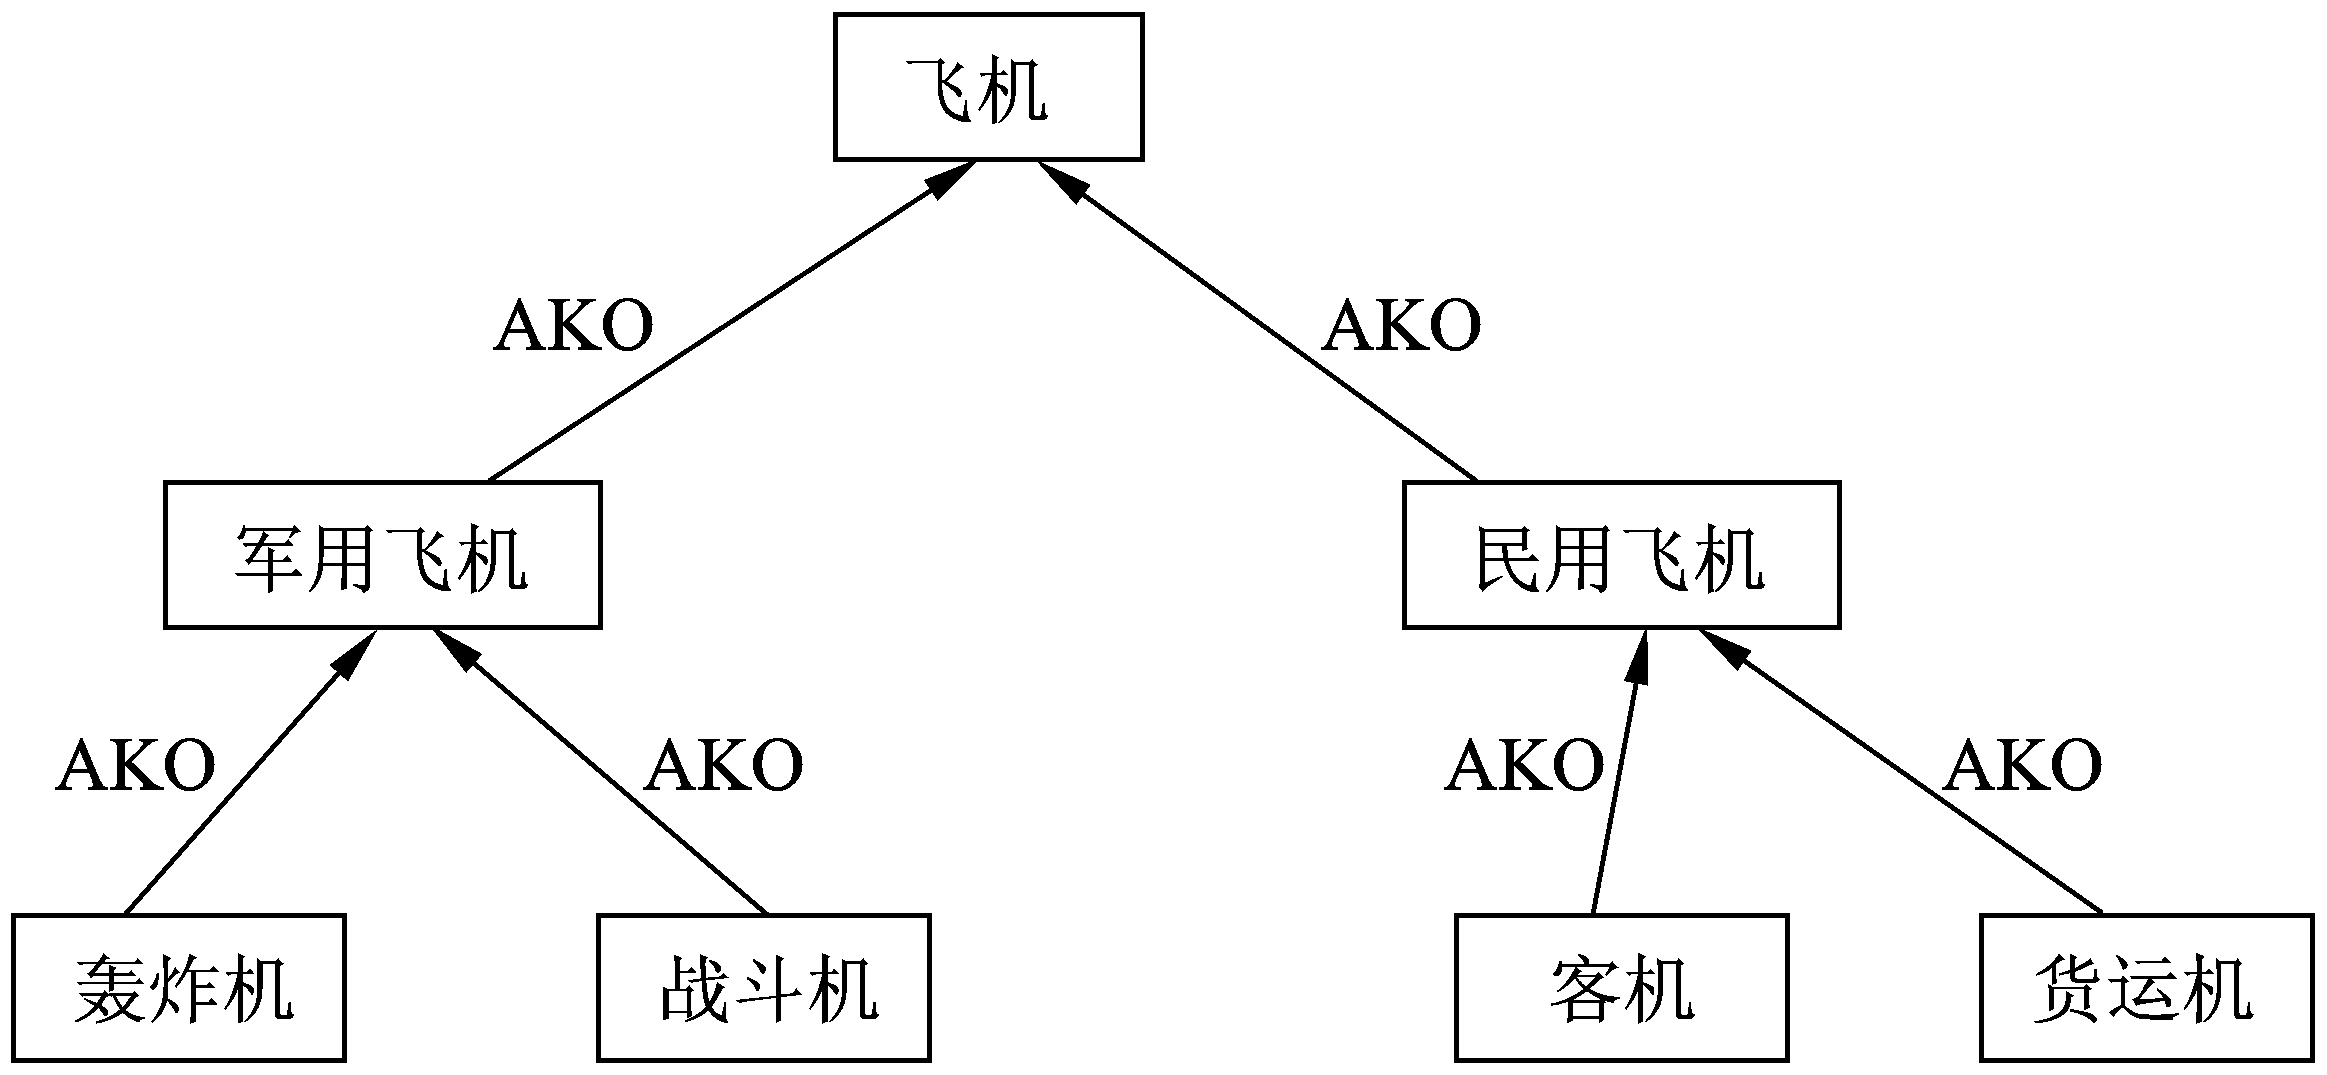
\includegraphics[width=0.4\textwidth]{YUYINETlizi01.png}
\caption{语义网络示例}
\label{YUYINETlizi01}
\end{figure}
\end{think}

%%%%%------------------------------------------
\begin{think}
  产生式表示法中事实和规则怎么表示?用产生式表示法设计一个医学知识库.
\end{think}

%%%%%------------------------------------------
\begin{think}
  以一所大学人员状况为例,说明语义网络的基本描述格式.
\end{think}

%%%%%------------------------------------------
\begin{think}
  框架表示法有什么特点?试构造一个描述你的卧室的框架系统.
\end{think}

%%%%%------------------------------------------
\begin{think}
  八数码问题也称为九宫问题. 在$3\times 3$的棋盘,摆有八个棋子,每个棋子上标有1~8的某一数字,不同棋子上标的数字不相同. 棋盘上还有一个空格,与空格相邻的棋子可以移到空格中.
  要求解决的问题是,给出一个初始状态和一个目标状态,找出一种从初始状态转变成目标状态的移动序列.
\end{think}

%\begin{figure}[H]
%\centering
%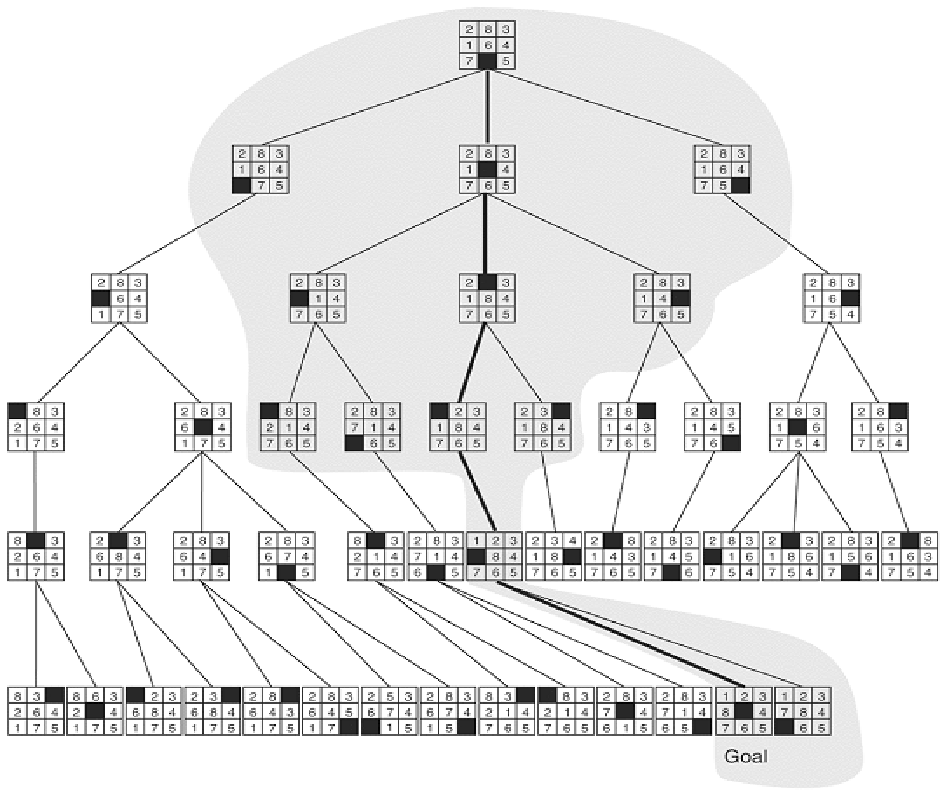
\includegraphics[width=0.6\textwidth]{Bashumalizi01.png}
%\caption{8数码问题的解树}
%\label{Bashumalizi01}
%\end{figure}

%%%%%------------------------------------------
\begin{custom}[explorecolor]{探索}
基于web的动物识别系统

    1. 实验目的

    理解和掌握产生式知识表示方法及产生式系统的基本过程, 能够利用Web编程技术建立一个基于产生式知识表示的简单的智能系统.

    2. 实验环境

    (1) 硬件环境: 网络环境中的微型计算机.

    (2) 软件环境: Windows操作系统, 任选一种网络编程语言和数据库管理系统.

    3. 实验要求

    (1) 以本书第2章动物识别产生式系统的规则为知识库(也可增加规则), 采用正向推理或逆向推理方式.

    (2) 以选定的数据库管理系统建立知识库, 用选定的网络编程语言按B/S模式开发一个具有解释功能的智能系统.

    (3) 提交完整的软件系统和相关文档, 包括源程序和可执行程序.
\end{custom}
